\documentclass[twocolumn]{article}

\usepackage{geometry}
\geometry{textwidth = 18cm,textheight = 24cm}

\usepackage{cite}
\usepackage{caption}
\usepackage{graphicx}
\usepackage{amsmath}
\usepackage{amssymb}
%\usepackage{braket}
\usepackage{textcomp}
%\usepackage{lmodern}
\usepackage{authblk}
\usepackage{datetime}
\usepackage{gensymb}
\usepackage{wrapfig}
%\usepackage[usenames,dvipsnames,svgnames,table]{xcolor}
\usepackage{booktabs}
%\usepackage{appendix}

%\usepackage[switch,columnwise]{lineno}
%\linenumbers

\newcommand{\onlinecite}[1]{\hspace{-1 ex} \nocite{#1}\citenum{#1}} 

\let\OLDthebibliography\thebibliography
\renewcommand\thebibliography[1]{
  \OLDthebibliography{#1}
  \setlength{\parskip}{0pt}
  \setlength{\itemsep}{0pt plus 0.3ex}
}
  
\title{Modeling Loop Neurons as Systems of Leaky Integrators}
\author[1]{\Large{NIST Physics and Hardware for Intelligence Project}
\\
\textit{\large{National Institute of Standards and Technology}}
\\
\vspace{-0.2em}
\textit{\large{325 Broadway, Boulder, CO, USA, 80305}}
\\
\vspace{-0.2em}
\textit{\large{jeffrey.shainline@nist.gov}}
}
\date{\today}%\today

\begin{document}

\twocolumn[
  \begin{@twocolumnfalse}
    \maketitle
    \begin{abstract}
At present, this document is a rough outline of the paper we shall write. After an introduction, we explore how superconducting optoelectronic synapses can be modeled as leaky integrators. We compare and contrast synapses with one, two, and three JJs. Then we show how these can be coupled to neurons in what is considered a point neuron: all synapses connect directly to the cell body without dendrites. We show how a point neuron can be used to represent the overall brightness of a nine-pixel image. The leaky integrator model of synapses and point neurons is compared to spice models to quantify accuracy. It is found that capturing the SPD response is currently limiting accuracy. Next we discuss dendrites and show that they can also be modeled as leaky integrators with a treatment that is nearly identical to synapses. We again compare to spice to quantify accuracy. We demonstrate how neurons with a dendritic arbor can be used to represent additional information in nine-pixel images such as vertical or horizontal bars, motion, and character classification. Finally we consider the ability of superconducting optoelectronic loop neurons to achieve subthreshold oscillations. By extending the synaptic or dendritic leak to complex values, the same model can be used to represent neuronal components that oscillate as they decay. Physically oscillation is accomplished with the inclusion of a capacitor along with the inductor and resistor in a synaptic or dendritic integration loop. 
    \vspace{3em}
    \end{abstract}
  \end{@twocolumnfalse}
]

\setcounter{tocdepth}{1}
\setcounter{secnumdepth}{4}
\tableofcontents

\section{\label{sec:introduction}Introduction}
The computations performed by superconducting optoelectronic loop neurons are accomplished by circuits comprising single-photon detectors, Josephson junctions, and mutual inductors. These devices are most commonly modeled with SPICE circuit simulations carried out on a picosecond time scale to accurately capture the dynamics of the Josephson junctions. Simulation of networks of large numbers of these neurons become computationally intensive. From the perspective of the neural system, the picosecond dynamics of the JJs are not important, and one would prefer to treat each synapse, dendrite, and neuron as an input-output device with a model that accurately captures the circuit dynamics on the nanosecond to microsecond time scales while not explicitly treating the picosecond behavior of the underlying circuit elements.

Here we introduce a phenomenological model of loop neurons and their constitutive elements that accurately captures the transfer characteristics of the circuits without solving the underlying circuit equations. Each synapse and dendrite is treated with a single, first-order ordinary differential equation that describes the output of the element as a function of its inputs and instantaneous internal state. These equations take the standard form of a leaky integrator with a nonlinear driving term. Each neuron performs passive summation of its synaptic and dendritic inputs. When the sum of the inputs reaches threshold, the neuron produces a spike. Refraction is treated with the same formalism as a strong inhibitory synapse receiving the neuron's spikes and directly contacting the neuron's cell body. When full circuit simulations are conducted, each synapse or dendrite require solving a system of seven equations at each time step, and time steps of 1\,ps are typical. The model presented here reduces the number of equations for each synapse or dendrite to one and allows simulation with time steps of 1\,ns. 

We begin by motivating the form of the model based on circuit considerations. We then describe the means by which the form of the driving term in the leaky integrator is obtained. Error is quantified by comparison to full circuit simulations, and convergence is investigated as a function of time step size. Point neurons are considered to test the synaptic equations. Dendrites are treated next, and the similarity between synaptic and dendritic circuits permits a treatment with a similar form of leaky integrator equation. Dendritic accuracy is quantified, and an example of a neuron with a dendritic arbor is presented to illustrate the utility of the model. Throughout the work we compare and contrast loop neurons with their biological counterparts. 

\section{\label{sec:leaky_integrators}Leaky Integrators}
Several aspects of biological neurons are commonly modeled by leaky integrator equations. For example, the membrane potential may be treated with an ODE of the form
\begin{equation}
\label{eq:leaky_integrator}
\frac{dV(t)}{dt} = f_{\mathrm{in}}(t)-\frac{V(t)}{\tau},
\end{equation}
where $V$ represents the membrane potential, $\tau$ is the leak rate of charge off the membrane capacitor, and $f_{\mathrm{in}}(t)$ represents an arbitrary time-varying input to the integrator due to synaptic and dendritic input currents. The leaky integrate-and-fire (LIF) model treats a system that follows Eq.\,\ref{eq:leaky_integrator}, but is also subject to the rule that when $V(t)$ reaches a threshold $\theta$, the neuron produces an action potential, and the value of $V(t)$ is set to a base value $V_0$. Additionally, standard LIF treatments commonly enforce an absolute refractory period wherein $V(t)$ is forced to remain below $\theta$ for some time $\tau_{\mathrm{ref}}$, or a relative refractory period wherein the magnitude of $\theta$ is temporarily increased.

Equation \,\ref{eq:leaky_integrator}, supplemented with thresholding, reset, and refraction, captures essential features of biological neurons and widely employed in computational neuroscience. The LIF model has also become the \textit{de facto} standard for artificial neural systems. Neurons governed by this model have several important attributes for information processing. First, they perform a sliding temporal summation, so their present state contains information regarding the recent activities of their synaptic and dendritic inputs. Second, the existence of a threshold, and the production of a spike upon reaching threshold from below, amounts to a logical operation mapping multiple inputs to one output. The information processing performed by a single LIF neuron can be summarized by a signal in/activity out transfer function like those shown in Fig.\,\ref{fig:leaky_integrator}. The presence of a non-zero threshold causes the transfer function to have a non-zero turn-on point, and refraction introduces a maximum firing rate, causing the transfer function to roll over at strong inputs. This non-linear transfer function ensures the neuron outputs different information than the sum of its inputs, and hence it computes.
%\begin{figure}[h!]
%\centering
%\includegraphics[width=8.6cm]{_01__leaky_integrator.pdf}
%\captionof{figure}{\label{fig:leaky_integrator}}
%\end{figure}

While LIF neurons are useful for computation, it is not obvious their specifications render them optimal for any type of information processing. Nor does it appear that the LIF model of point neurons captures many of the subtleties of biological neurons that may augment their ability to glean information from their inputs. Nevertheless, the LIF model gives us a useful starting point in both computational neuroscience and development of hardware for artificial intelligence. Efforts to devise neuromorphic hardware must respond to two influences. Artificial neural systems must maintain a reasonably close resemblance to their biological forbears so that the complex information processing capable of cognition can be manifest in technological systems. This drives the designer to seek behavior similar to LIF. At the same time, realization of artificial neural systems in hardware requires us to respect the physics as well as practical fabrication and operation constraints of the devices being utilized. Together these influences provide guide rails as well as opportunities. We know we wish to start with something like leaky integrators, and we know our devices will encounter constraints that shape the ways in which they can be used, but we can also be on the lookout for means to augment what can be achieved with biological hardware.

Superconducting optoelectronic loop neurons are one such endeavor that aspires to realize artificial neural systems with complexity comparable to the human brain. We next summarize the salient features of loop neurons before exploring the mathematical properties, which bear a strong resemblance to Eq.\,\ref{eq:leaky_integrator}, but also offer opportunities for augmentation. One of the goals of developing the phenomenological model presented here is to elucidate similarities and differences between loop neurons and well-studied LIF neurons. 

\section{\label{sec:overview_of_loop_neurons}Overview of Loop Neurons}
We have introduced the concepts of loop neurons in a number of papers, and we have demonstrated many of the principles experimentally. This background is summarized in Appendix \ref{apx:background}. 

Schematic diagrams of two types of loop neuron are shown in Fig.\,\ref{fig:schematic}. Figure \ref{fig:schematic}(a) shows the point-neuron concept \cite{sh2018,sh2019_jap}, while Fig.\,\ref{fig:schematic}(b) shows the concept when a dendritic tree is included \cite{sh2019_jstqe}. In these neurons, integration, synaptic plasticity, and dendritic processing are implemented with inductively coupled loops of supercurrent. It is due to the prominent role of superconducting storage loops that we refer to devices of this type as loop neurons. 

Operation of loop neurons is as follows. Photons from upstream neurons are received by a superconducting single-photon detector (SPD) at each synapse. Using a Josephson junction (JJ) in parallel with an SPD, synaptic detection events are converted into an integrated supercurrent which is stored in a superconducting loop. The circuit diagram of a synapse is shown in Fig.\,\ref{fig:circuits}(a). The amount of current that gets added to the integration loop during a photon detection event is determined by the synaptic weight. The synaptic weight is dynamically adjusted by another circuit combining SPDs and JJs, and all involved circuits are analog. When the integrated current of a given neuron reaches a (dynamically variable) threshold, an amplification cascade begins, resulting in the production of light from a waveguide-integrated semiconductor light emitter. The photons thus produced fan out through a network of dielectric waveguides and arrive at the synaptic terminals of other neurons where the process repeats. 

In loop neurons, a synapse consists of an SPD in parallel with a JJ (which together transduce photons to supercurrent), and a superconducting loop, which stores a current proportional to the number of detected photon arrival events. This loop is referred to as the synaptic integration (SI) loop. Within each neuron, the loops of many synapses are inductively coupled to a larger superconducting loop, referred to as the neuronal receiving (NR) loop, thereby inducing an integrated current proportional to a weighted sum of the currents in all the neuron's synapses. When the current in this NR loop reaches a threshold, the neuron produces a current pulse in the form of one or more flux quanta. This current is amplified and converted to voltage to produce photons from a semiconductor $p-i-n$ junction.

The currents in the synaptic and neuronal loops are analogous to the membrane potential of biological neurons \cite{daab2001,geki2002}, and the states of flux in these loops are the principal dynamical variables of the synapses and neurons in the system. Inhibitory synapses can be achieved through mutual inductors with the opposite sign of coupling. Dendritic processing can be implemented straightforwardly by adding intermediate mutually inductively coupled loops between the synaptic and neuronal loops. Synapses can be grouped on dendritic loops capable of local, nonlinear processing and inhibition. Neurons with multiple levels of dendritic hierarchy can be implemented as multiple stages of integrating loops. The temporal scales of the SI and DI loops can be set with $L/r$ time constants. I expect all synaptic and dendritic signals to leak, enabling fading memory of recent activity. Also, I hypothesize that the ability to achieve a diversity of time constants through synapses and dendrites with many $L/r$ time constants will be advantageous, and I would like to investigate this in numerical studies.

Synaptic memory is also implemented based on the stored flux in a loop, referred to as the synaptic storage (SS) loop. The state of flux in the SS loop determines the current bias to the synaptic receiver circuit discussed above. This current bias is the synaptic weight. In contrast to the SI and DI loops, the SS loop is intended to store long-term memory, and therefore I do not expect to add a resistance to this loop. If the SS loop is created with a superconducting wire of high inductance, the loop can hold many discrete states of flux, and therefore can implement many synaptic weights, if desired. Synapses with a pseudo-continuum of hundreds of stable synaptic levels between minimal and maximal saturation values are possible. Transitions between these levels can be induced based on the relative arrival times of photons from the pre-synaptic and post-synaptic neurons, thereby establishing a means for spike-timing-dependent plasticity with one photon required for each step of the memory-update process. Binary synapses are also possible, and just as we expect a diversity of $L/r$ time constants to be advantageous for tracking activity over time, we expect a diversity of synapses raging from binary to multistable to be advantageous for striking a balance between adaptability and long-term memory retention.

\begin{figure}[h!]
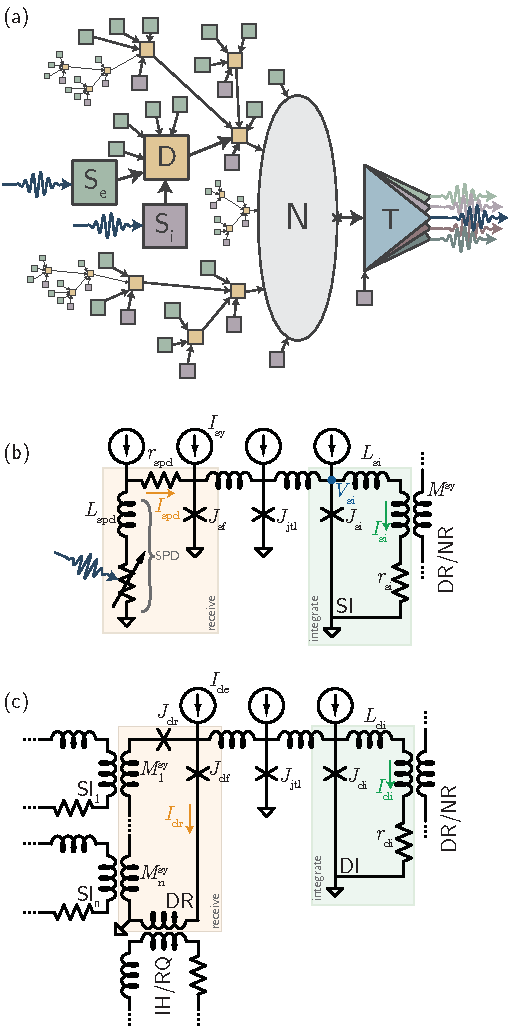
\includegraphics[width=8.6cm]{figures/_02__schematic__circuits.pdf}
\captionof{figure}{\label{fig:schematic__circuits}(a) Schematic. (b) Circuits. %Two schematics of loop neurons. (a) A point loop neuron (no dendritic tree) showing excitatory ($\mathsf{S_e}$) and inhibitory ($\mathsf{S_i}$) synapses, as well as synaptic weight update circuits ($\mathsf{W}$). The wavy, colored arrows are photons, and the straight, black arrows are electrical signals. The synapses receive signals as faint as a single photon and add supercurrent to an integration loop. Upon reaching threshold, a signal is sent to the transmitter circuit ($\mathsf{T}$), which produces a photon pulse. Some photons from the pulse are sent to downstream synaptic connections, while some are used locally to update synaptic weights. (b) A loop neuron with an elaborate dendritic tree. The complex structure consists of excitatory and inhibitory synapses that feed into dendrites ($\mathsf{D}$). Each dendrite performs computations on the inputs and communicates the result to other dendrites for further processing or on to the cell body of the neuron ($\mathsf{N}$). The neuron itself acts as the final thresholding stage, and when its threshold is reached, light is produced by the transmitter ($\mathsf{T}$), which is routed to downstream synaptic connections.
}
\end{figure}

\section{\label{sec:synapses}Synapses as Leaky Integrators}
The objective of this section is to express the output of a synapse as a function of the input without solving the explicit circuit equations. The synapse under consideration in shown in Fig.\,\ref{fig:syn__circuit__rate_array}(a). We begin with the hypothesis that the circuit can be modeled as a leaky integrator, with the primary dynamical quantity being the integrated current circulating in the SI loop, and a drive term resulting from photon detection events. When the SPD receives a photon, its bias current, $I_{\mathrm{spd}}$, is diverted to the synaptic firing junction, $J_{\mathrm{sf}}$. If the combination $I_{\mathrm{spd}}+I_{\mathrm{sy}}$ exceeds the critical current of $J_{\mathrm{sf}}$, a series of fluxons will be generated. At the circuit level, $J_{\mathrm{sf}}$ will first produce a fluxon. The current from this fluxon will drive $J_{\mathrm{jtl}}$ above $I_c$, causing it to produce a fluxon. Likewise, this fluxon will drive $J_{\mathrm{si}}$ above $I_c$, and the fluxon thus produced will be added to the SI loop, increasing the value of the dynamical variable of interest. After this fluxon has increased $I_{\mathrm{si}}$, if $J_{\mathrm{sf}}$ is still being held above $I_c$ by the combination of $I_{\mathrm{spd}}$ and $I_{\mathrm{sy}}$, another fluxon will be produced and propagate through the circuit in the same manner. Depending on the strength of the synaptic weight and the flux storage capacity of the SI loop, a single synapse event may add anywhere from a few fluxons up to over one thousand fluxons to the SI loop. Each fluxon adds $\Delta I_{\mathrm{si}} = \Phi_0/L_{\mathrm{si}}$ to the circulating current in the SI loop. $\Phi_0 = h/2e \approx 2\times10^{-15}\mathrm{V}\cdot\mathrm{s}$ is the magnetic flux quantum. The current in the SI loop decays with time constant $\tau_{\mathrm{si}} = L_{\mathrm{si}}/r_{\mathrm{si}}$. Given this picture of circuit operation, we can see a path toward modeling the synapse as a leaky integrator. The driving term is determined by the rate of fluxon production, and the leak term is governed by $\tau_{\mathrm{si}}$.

\subsection{Synapses with one Josephson Junction}

This description of the operation of the circuit is based on well-known properties of Josephson junctions within the formalism of the resistively and capacitively shunted junction (RCSJ) model \cite{vatu1998,ka1999,ti1996}. The relevant behavior derives from the fact that a JJ will produce a voltage fluxon after a time $t_{\mathrm{fq}}$ determined by the relation
\begin{equation}
\label{eq:jj__fluxon_production}
\int_0^{t_{\mathrm{fq}}}V(t)dt = \Phi_0 \rightarrow r^{\mathrm{fq}} = 1/t^{\mathrm{fq}}.
\end{equation}
The voltage $V(t)$ across the junction is related to the current bias by a relation of the form

\begin{equation}
\label{eq:jj__current_voltage}
V^{\mathrm{sf}}(I^{\mathrm{sf}}) = V_0\left[ \left( \frac{I^{\mathrm{sf}}}{I_c-I_r} \right)^{\mu_1} - 1 \right]^{\mu_2}.
\end{equation} 
where the values $\mu_1$, $\mu_2$, and $V_0$ depend on the specific parameters of the shunt resistance and capacitance in the RCSJ model. For the junctions considered here, $I_r = 1.1768$\,\textmu A is the reset current associated with hysteresis on $J_{\mathrm{sf}}$ due to the fact that $\beta_c = 0.95 > 0$. $\mu_1 = 3.464271$, $\mu_2 = 0.306768$, and $V_0 = 233.966$\,\textmu V. From Eqs.\,{eq:jj__fluxon_production} and \ref{eq:jj__current_voltage} we can obtain $r^{\mathrm{fq}}$. In the case where $I^{\mathrm{sf}}$ is slowly varying compared to $t^fq$, $ r^{\mathrm{fq}} = V^{\mathrm{sf}}/\Phi_0$. 

%The voltage across each JJ in the circuit is evolving in time as the current biases change, and when any junction produces a fluxon, the adjacent junctions experience a new bias condition due to the current of that fluxon. The temporal envelopes of these current pulses are on the picosecond scale. Based on Eqs.\,\ref{eq:jj__fluxon_production} and \ref{eq:jj__current_voltage} one may attempt to construct an analytical model of the rate of fluxon generation. However, accurate determination of the fluxon generation rates depends on accurate determination of the currents $I(t)$ which requires consideration of picosecond timescales. 

\begin{figure*}[htb]
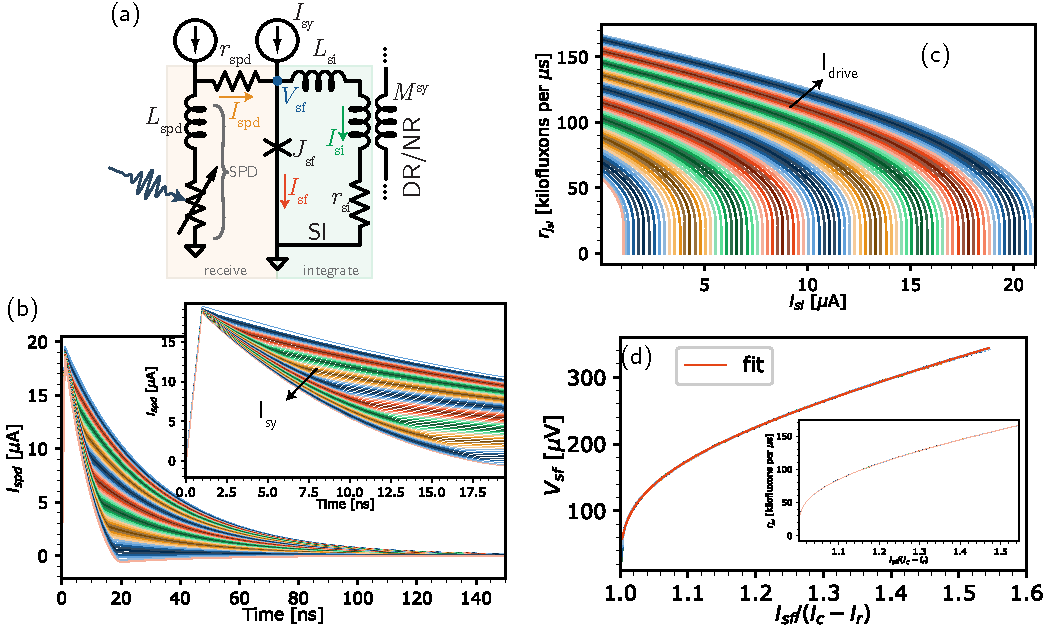
\includegraphics[width=17.2cm]{figures/_03__syn__1jj__circuit__rate_array.pdf}
\captionof{figure}{\label{fig:syn__circuit__rate_array}(a) Circuit diagram of synapse. (b) Also include fluxon generation detail. (c) Rate array.}
\end{figure*}
We do not wish to consider such timescales nor fluxon-generation dynamics when simulating large networks with many synapses. But these circuit considerations provide sufficient insight to postulate a form for a leaky integrator ODE that will accurately model the input-output relationship of a synapse on longer timescales. Consider a synaptic model of the form 
\begin{equation}
\label{eq:leaky_integrator__SI_loop}
\frac{dI^{\mathrm{si}}(t)}{dt} = r^{\mathrm{fq}}\left(I^{\mathrm{sf}}(t)\right) I^{\mathrm{fq}}-\frac{I^{\mathrm{si}}(t)}{\tau^{si}}.
\end{equation}
where $r^{\mathrm{fq}}(I^{\mathrm{sf}},I^{\mathrm{si}})$ represents the rate at which fluxons are added to the SI loop as a function of the total current across the synaptic firing junction, $I^{\mathrm{sf}}$, as well the current circulating in the SI loop, $I^{\mathrm{si}}$. $I^{\mathrm{fq}} = \Phi_0/L^{\mathrm{si}}$ is the current added to the SI loop with each fluxon. The flux-induced current $I^{\mathrm{si}}$ circulates in the SI loop in a manner that counters the bias to $J^{\mathrm{si}}$. It is this counter-biasing that causes the SI loop to saturate as a function of $I^{\mathrm{si}}$. When $I^{\mathrm{si}}$ becomes sufficiently large, the fluxon generated by $J^{\mathrm{jtl}}$ does not provide enough current to drive $J^{\mathrm{si}}$ above $I_c$, and the stored flux in the SI loop must decay before subsequent synapse events can add to the integrated signal.

Based on these considerations, we expect that $r^{\mathrm{fq}}(I^{\mathrm{sf}},I^{\mathrm{si}})$ will grow monotonically with $I^{\mathrm{sf}}$, and decrease monotonically with $I^{\mathrm{sy}}$. We are treating $r^{\mathrm{fq}}$ as a continuous variable, although flux quanta are produced discretely. This approximation is valid for two reasons. First, typical SI loops can store the signals from hundreds to tens of thousands of fluxons, so the current added to the SI loop as a stream of fluxons enters grows in very small increments. Second, the highest firing frequencies of loop neurons are around 100\,MHz, so the dynamics of $I^{\mathrm{si}}$ are only relevant on time scales of 1\,ns and longer. Because fluxons are generated at rates in excess of 10\,GHz when $J^{\mathrm{sf}}$ is driven above $I_c$, treating $r^{fq}$ as a continuous function on nanosecond timescales is acceptable.

Completion of the model of a loop synapse as a leaky integrator now requires accurate determination of the function $r^{\mathrm{fq}}(I^{\mathrm{sf}},I^{\mathrm{si}})$. We have determined this function numerically through a simple series of circuit simulations using WRSpice \cite{wh1991}. In each simulation the total bias to the synaptic firing junction, $I^{\mathrm{sf}}$, was held constant at a value in excess of $I_c$. The value of $L^{\mathrm{si}}$ was chosen so the SI loop would saturate within a few tens of nanoseconds after receiving on the order of 1000 fluxons. $\tau^{\mathrm{si}}$ was set to infinity. Fluxons are evident as sharp voltage pulses across each JJ in the circuit, as shown in Fig.\,\ref{fig:to_be_added}, and the rate of fluxon generation can be directly calculated from the time between fluxons. By calculating this rate through the time course of the simulation as $I^{\mathrm{si}}$ grows, one can obtain $r^{\mathrm{fq}}$ as a function of $I^{\mathrm{si}}$. By running many such simulations for multiple values of $I^{\mathrm{sf}}$, a complete determination of $r^{\mathrm{fq}}(I^{\mathrm{sf}},I^{\mathrm{si}})$ can be obtained. In the present study, 53 simulations with 53 values of $I^{\mathrm{sf}}$ from $I_c$ to $I^{\mathrm{spd}}$ we conducted. The resultant function $r^{\mathrm{fq}}$ is plotted in Fig.\,\ref{fig:syn__circuit__rate_array}. We refer to this numerical construction as the synaptic rate array. Determination of the rate array completes the specification of the synaptic leaky-integrator model as given in Eq.\,\ref{eq:leaky_integrator__SI_loop}.

We assess the accuracy of this model based on its ability to reproduce the behavior of synapse circuits under a wide range of conditions. To conduct this comparison, WRSpice was used to simulate synaptic circuits for a broad range of values of synaptic bias current, $I^{\mathrm{sy}}$; SI loop inductance (storage capacity), determined by $L^{\mathrm{si}}$ ($\beta_L = 2\pi L I_c/\Phi_0$); and SI loop storage time, $\tau^{\mathrm{si}}$. These circuits were simulated in the presence of an arbitrary input pulse sequence as would be received by the SPD in the presence of afferent synaptic activity, so the current drive, $I^{\mathrm{spd}}$, was a sequence of exponential pulses, as shown in Fig.\,\ref{fig:syn__circuit__rate_array__add_drive_signal}. The leaky-integrator model under consideration, Eq.\,\ref{eq:leaky_integrator__SI_loop}, was implemented numerically with the Euler method. Comparison between circuit simulations and the model are shown in Figs.\,\ref{fig:syn__cmpr__vary_Isy}-\ref{fig:syn__cmpr__vary_tausi} for twelve synaptic configurations covering broad ranges of $I^{\mathrm{sy}}$, $L^{\mathrm{si}}$, and $\tau^{\mathrm{si}}$. To quantify the accuracy, we use a $\chi^2$ of the form
\begin{equation}
\label{eq:chi_squared}
\chi^2 = \frac{\int \left|I^{\mathrm{si}}_{\mathrm{spice}}(t) - I^{\mathrm{si}}_{\mathrm{ode}}(t)\right|^2 dt}{\int \left|I^{\mathrm{si}}_{\mathrm{spice}}(t)\right|^2 dt}.
\end{equation}
Convergence as a function of time step, $dt$ is shown in Fig.\,\ref{fig:syn__error_vs_dt}. Accuracy of $10^{-3}$ is easily obtained with nanosecond time steps for all cases, and in some cases accuracy at the $10^{-5}$ level is achieved. 


\begin{figure*}[htb]
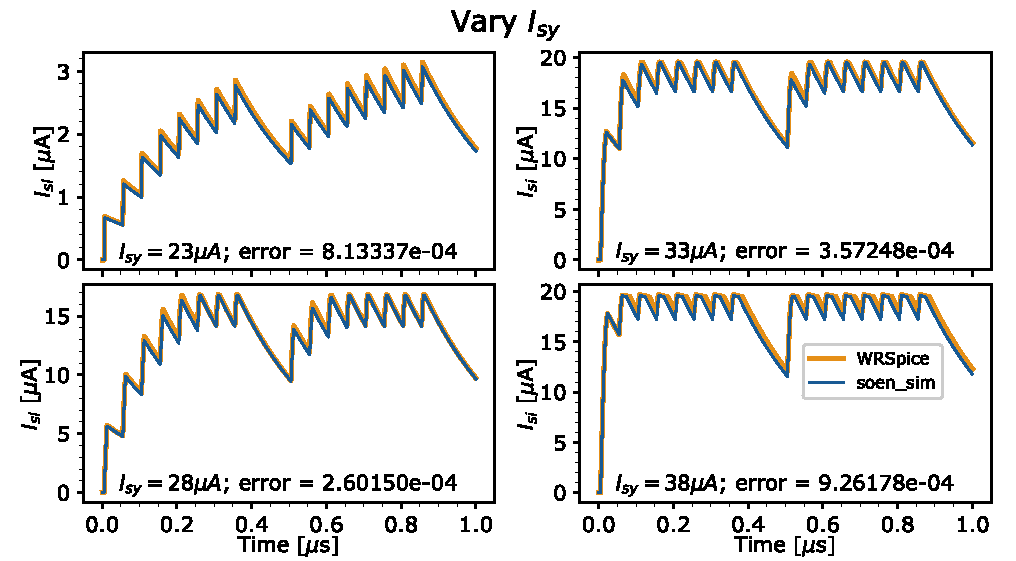
\includegraphics[width=17.2cm]{figures/_04__syn__cmpr__vary_Isy.pdf}
\captionof{figure}{\label{fig:syn__cmpr__vary_Isy}Varying the synaptic bias current, $I_{\mathrm{sy}}$.}
\end{figure*}

\begin{figure*}[htb]
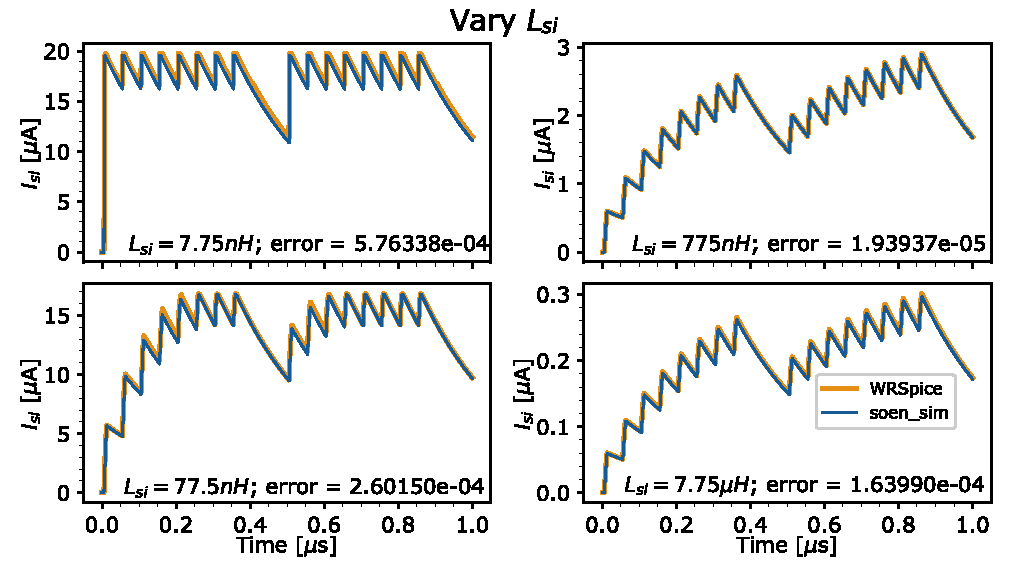
\includegraphics[width=17.2cm]{figures/_04__syn__cmpr__vary_Lsi.pdf}
\captionof{figure}{\label{fig:syn__cmpr__vary_Lsi}Varying the SI loop inductance, $L_{\mathrm{si}}$.}
\end{figure*}

\begin{figure*}[htb]
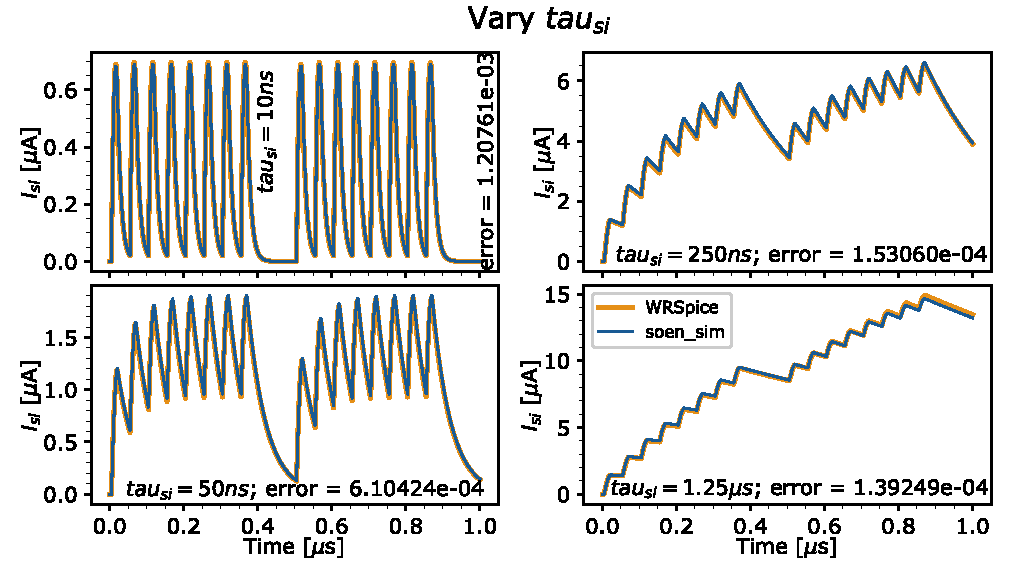
\includegraphics[width=17.2cm]{figures/_04__syn__cmpr__vary_tausi.pdf}
\captionof{figure}{\label{fig:syn__cmpr__vary_tausi}Varying the SI loop leak rate, $\tau_{\mathrm{si}}$.}
\end{figure*}

\begin{figure*}[htb]
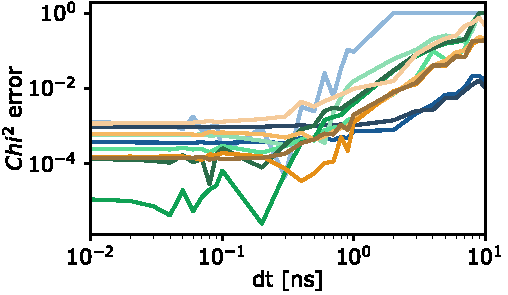
\includegraphics[width=17.2cm]{figures/_05__syn__error_vs_dt.pdf}
\captionof{figure}{\label{fig:syn__error_vs_dt}Error vs dt.}
\end{figure*}

An important limitation of the one-JJ synapse is illustrated in Fig.\,\ref{fig:syn__1jj__Isisat_vs_Isy}. Not only does the amount of current added to the SI loop with each synapse event depend on $I_{\mathrm{sy}}$, the value of current at which the SI loop saturates and further synaptic activity cannot be integrated also depends on $I_{\mathrm{sy}}$.  
\begin{figure}[htb]
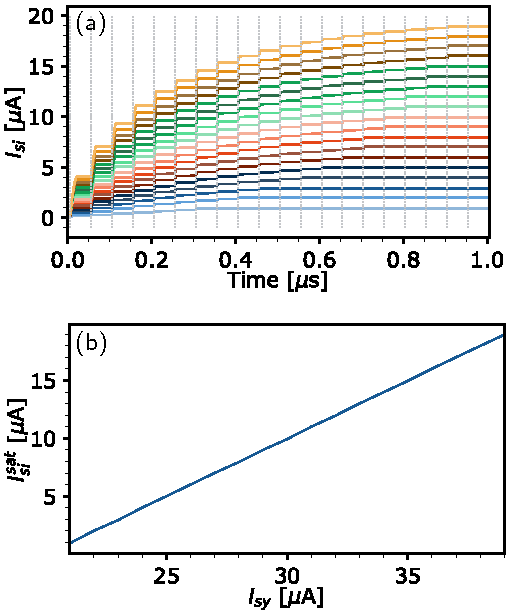
\includegraphics[width=8.6cm]{figures/_05__syn__1jj__Isisat_vs_Isy.pdf}
\captionof{figure}{\label{fig:syn__error_vs_dt}SI loop saturation versus synaptic bias current for the one-JJ synapse.}
\end{figure}
While this characteristic of the one-JJ synapse may be acceptable in certain circumstances, we would like to explore the possibility of decoupling the amplitude of each synapse event from the integration capacity of the SI loop. This behavior can be accomplished by adding an additional JJ to the synapse.

\subsection{Synapses with Two or Three Josephson Junctions}
\begin{equation}
\label{eq:leaky_integrator__SI_loop}
\frac{dI^{\mathrm{si}}(t)}{dt} = r^{\mathrm{fq}}\left[I^{\mathrm{sf}}(t),I^{\mathrm{si}}(t)\right] I^{\mathrm{fq}}-\frac{I^{\mathrm{si}}(t)}{\tau^{si}}.
\end{equation}

\begin{figure*}[htb]
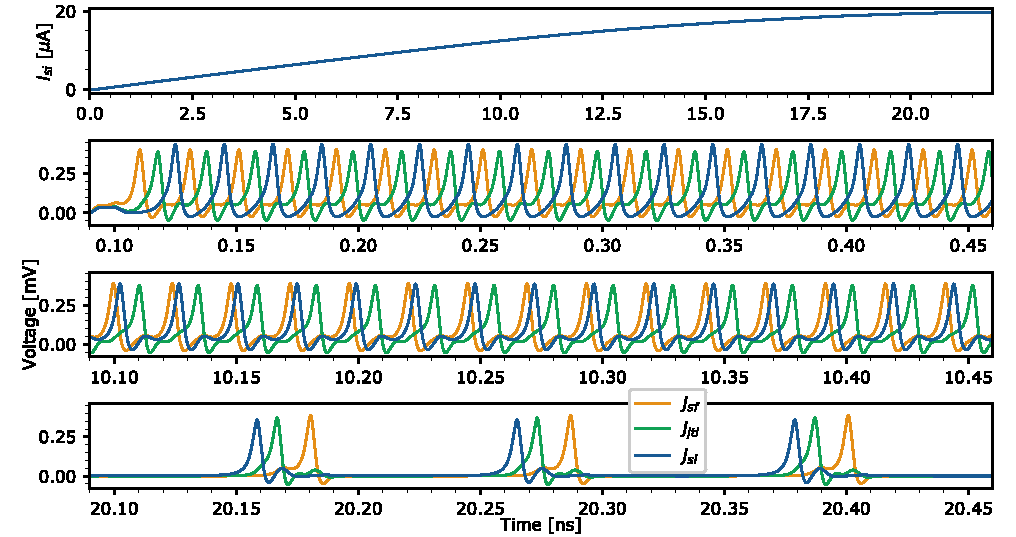
\includegraphics[width=17.2cm]{figures/_03__syn__fq_peaks.pdf}
\captionof{figure}{\label{fig:syn__fq_peaks}Caption.}
\end{figure*}

\begin{figure}[htb]
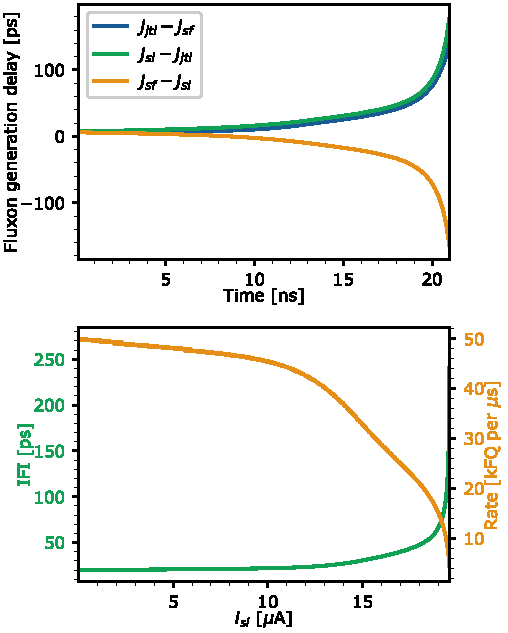
\includegraphics[width=8.6cm]{figures/_03__syn__fq_delay_and_rate.pdf}
\captionof{figure}{\label{fig:syn__fq_delay_and_rate}Caption.}
\end{figure}

\section{\label{sec:point_neurons}Point Neurons}
Many models of neurons assume the the neuron cell body sums the inputs from all synapses and compares this sum to a threshold. Such a construction is referred to as a point neuron, in contrast to more elaborate neuron models that account for the intermediate signal processing of the dendritic arbor. Having completed the model of synapses as leaky integrators, we are in a position to treat point neurons. Dendrites will be considered subsequently.

%\begin{equation}
%\label{eq:I_nr}
%I^{nr}(t) = \sum_j m_j I_j^{si}(t).
%\end{equation}

\begin{equation}
\label{eq:I_nr__with_refraction}
I_i^{nr}(t) = m_i^{rs}I^{rs}(t)+\sum_j m_{ij} I_j^{si}(t).
\end{equation}

\begin{figure}[htb]
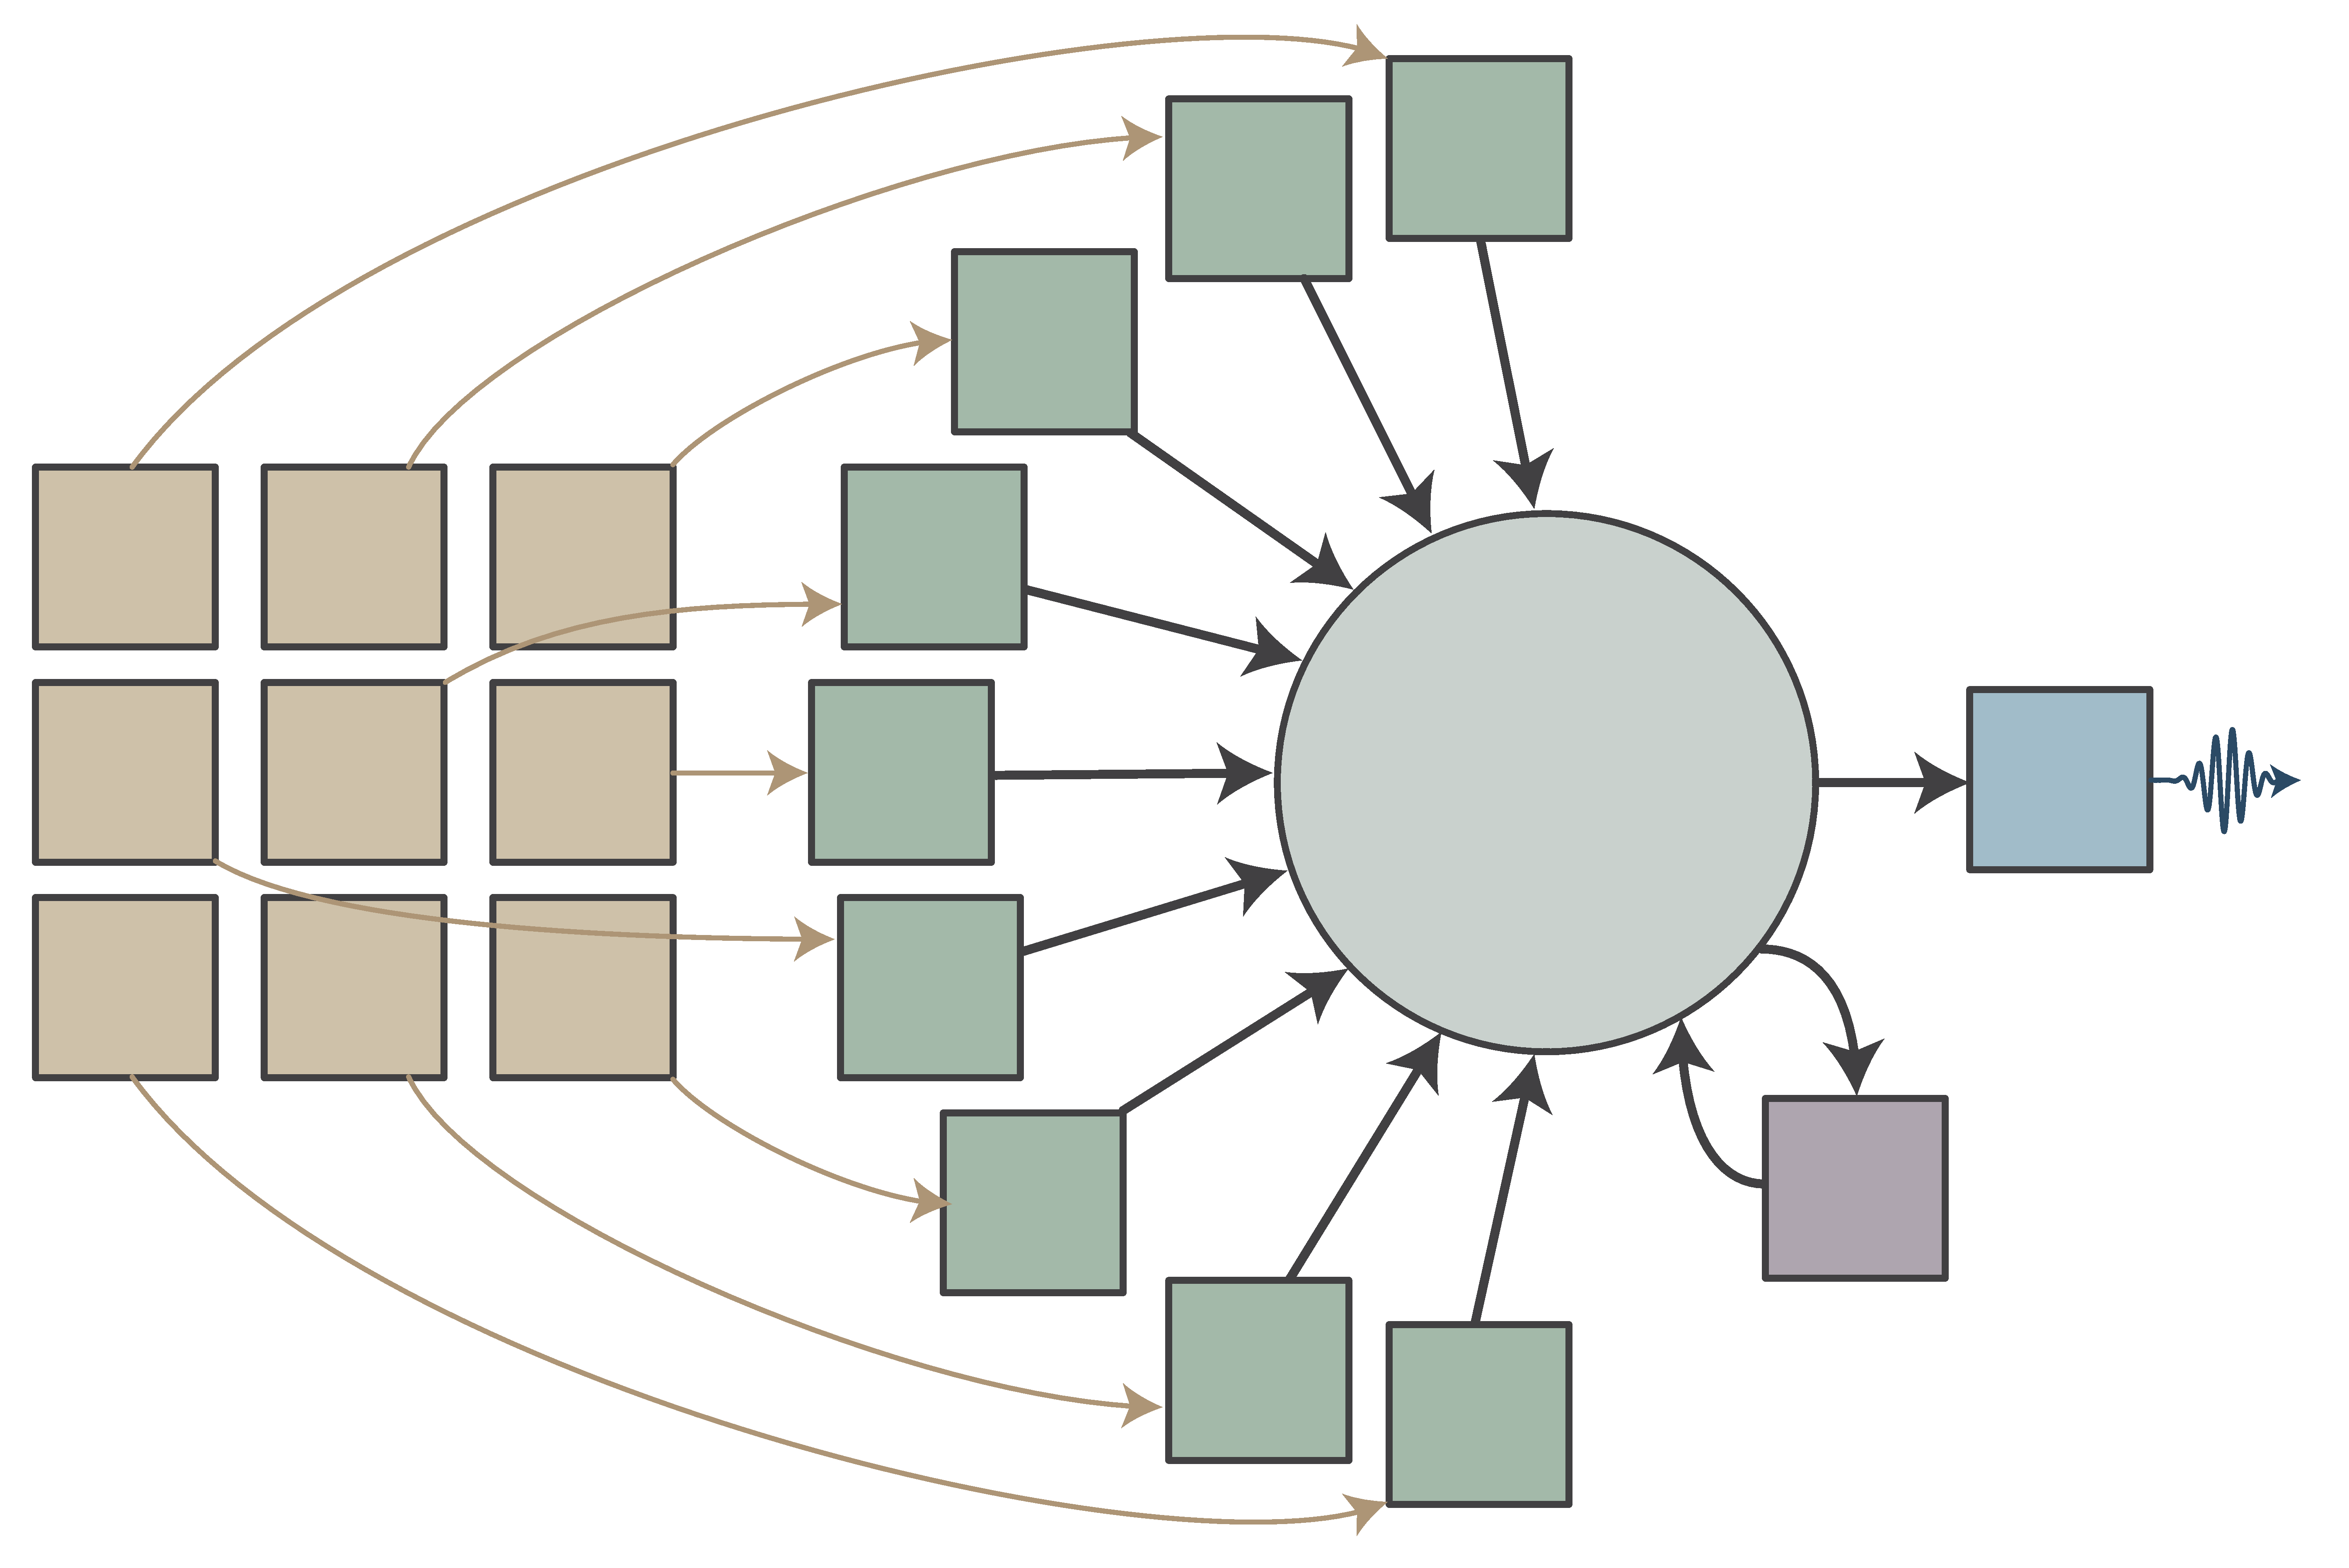
\includegraphics[width=8.6cm]{figures/_06__point_neuron__nine_pixel_schematic.pdf}
\captionof{figure}{\label{fig:point_neuron__nine_pixel_schematic}Nine pixel schematic.}
\end{figure}
 
%\begin{figure}[h!]
%\includegraphics[width=8.6cm]{figures/_07__point_neuron__transfer_functions.pdf}
%\captionof{figure}{\label{fig:point_neuron__transfer_functions}Point neuron transfer functions. (a) Rate. (b) Burst.}
%\end{figure}

\section{\label{sec:dendrites}Dendrites as Leaky Integrators}

\begin{equation}
\label{eq:leaky_integrator__SI_loop}
\frac{dI^{\mathrm{di}}(t)}{dt} = r^{\mathrm{fq}}\left[\sum_j I^{\mathrm{si}}_{j}(t),I^{\mathrm{di}}(t)\right] I^{\mathrm{fq}}-\frac{I^{\mathrm{di}}(t)}{\tau^{di}}.
\end{equation}

%\begin{equation}
%\label{eq:I_dr}
%\frac{dI^{di}(t)}{dt} = f\bigg(\sum_i m_i I_i^{si}(t),I^{di}(t)\bigg)-\frac{1}{\tau^{di}}I^{di}(t).
%\end{equation}
% 
%\begin{figure}[htb]
%\includegraphics[width=8.6cm]{figures/_08__dnd__circuit__rate_array.pdf}
%\captionof{figure}{\label{fig:dnd__circuit__rate_array}(a) Circuit diagram of dendrite. (b) Rate array.}
%\end{figure}

%\begin{figure}[htb]
%\includegraphics[width=8.6cm]{figures/_09__dnd__cmpr.pdf}
%\captionof{figure}{\label{fig:dnd__cmpr}Comparing to WR.}
%\end{figure}
 
%\begin{figure}[htb]
%\includegraphics[width=8.6cm]{figures/_10__dnd__error_vs_dt.pdf}
%\captionof{figure}{\label{fig:point_neuron__transfer_functions}Point neuron transfer functions. (a) Rate. (b) Burst.}
%\end{figure}

\section{\label{sec:dendritic_arbor}Neurons with a Dendritic Arbor}

%\begin{figure}[htb]
%\includegraphics[width=8.6cm]{figures/_11__arbor__bar_finder_schematic.pdf}
%\captionof{figure}{\label{fig:arbor__bar_finder_schematic}Bar finder schematic.}
%\end{figure}
%
%\begin{figure}[htb]
%\includegraphics[width=8.6cm]{figures/_12__arbor__bar_finder_data.pdf}
%\captionof{figure}{\label{fig:arbor__bar_finder_data}Bar finder data.}
%\end{figure}

\begin{figure}[htb]
\includegraphics[width=8.6cm]{figures/_13__arbor__classifier_schematic.pdf}
\captionof{figure}{\label{fig:arbor__classifier_schematic}Arbor classifier schematic.}
\end{figure}

\section{\label{sec:subthreshold_oscillations}Subthreshold Oscillations and Synchronization}

%\begin{figure}[h!]
%\includegraphics[width=8.6cm]{figures/_14__arbor__classifier_data.pdf}
%\captionof{figure}{\label{fig:arbor__classifier_data}Arbor classifier data.}
%\end{figure}

%\section{\label{sec:spike_response_model}The Spike Response Model}
%The spike response model (SRM) is a phenomenological model of neuron behavior that is complimentary to integrate-and-fire models. The approach leverages closed-form expressions for the response of the membrane potential to synaptic activity and production of action potentials. We can construct similar models based on loop neuron circuits to facilitate numerical analysis of loop neurons and networks.
%
%I have learned about SRM from the textbook called Spiking Neuron Models by Gerstner and Kistler \cite{geki2002}. From Gerstner and Kistler, pg. 102, the SRM is structured as follows. The state of neuron $i$ at time $t$ is described by a single variable, $u_i(t)$. In the absence of spikes, $u_i(t) = u_{\mathrm{rest}}$. The function
%\begin{equation}
%\label{eq:synaptic_response_kernel}
%\epsilon_{ij}(t-t_j^{(f)})
%\end{equation}
%describes the time course of the response to an incoming spike train. The function $\epsilon$ is referred to as the \textit{synaptic response kernel}, and $t_j^{(f)}$ is the full list of times at which a pulse leaving neuron $j$ was received at a synapse on neuron $i$. If $u_i(t)$ reaches threshold $\theta$, an output spike is triggered. The response of the variable $u_i(t)$ to the production of this action potential is modeled by the function
%\begin{equation}
%\label{eq:reset_kernel}
%\eta(t-\hat{t}_i),
%\end{equation}
%where $\hat{t}_i$ is the time of the last action potential produced by neuron $i$. The function $\eta$ is referred to as the \textit{reset kernel}. After firing, the evolution of $u_i(t)$ follows
%\begin{equation}
%\label{eq:spike_response_model}
%u_i(t) = \eta(t-\hat{t}_i)+\sum_j w_{ij}\sum_f \epsilon_{ij}(t-t_j^{(f)}).
%\end{equation}
%In biological neurons, $\epsilon$ may also depend on $\hat{t}_i$ due to physiological activity with the cell due to action potential creation. Such behavior is not native to loop neurons. It could be added if advantageous, but at present we neglect it from the model. The time between when neuron $j$ produces a pulse and when it is received by neuron $i$ is the delay, and we neglect delay in this work. One can also include a term to account for external drive that takes the form
%\begin{equation}
%\label{eq:external_drive}
%\int_0^{\infty}\kappa(t-\hat{t}_i,s)I^{\mathrm{ext}}(t-s)ds,
%\end{equation}
%but we also ignore this term and assume all external drives are input through synapses with response given by $\epsilon$.
%
%For the purpose at hand, we consider Eq.\,\ref{eq:spike_response_model} to represent the SRM for point neurons in a form that is most relevant to modeling loop neurons.
%
%\section{\label{sec:synapses}Phenomenological Model of Synapses}
%In loop neurons, the best model for the neuron as a whole may not be a leaky integrator, but rather a spike response model for each synapse, a leaky integrator ODE for each dendrite, and a summation for the signal present in the neuron. Let us begin to model loop neurons by modeling a synapse in isolation. Let us first consider a synapse in the context of a leaky integration model and proceed from there to reduce it to a closed-form expression for the synaptic response to a firing event. 
%
%In the circuit of Fig.\,\ref{fig:circuits}(a), the dynamical quantity that passes information to the rest of the neuron is the current circulating in the SI loop, $I_{\mathrm{si}}(t)$. Current is added to the loop when the synaptic firing junction, $J_{sf}$, is driven above the junction's critical current ($I_c$) by the redirection of current from the SPD to $J_{sf}$ during a synaptic firing event. Due to the nature of JJs, exceeding the $I_c$ of the junction results in the production of a series of fluxons. These fluxons are generated at a rate that is dependent on both the $I_c$ (which is static) and the current bias, $I_b$. The functional form of this current-dependent rate is not simple, in general, so we simply refer to the rate of production of flux quanta as $r_{fq}(I_b;t)$\footnote{In the case of junctions with damping parameter $\beta_c\ll 1$, there is a closed form expression: $r_{fq} = R\sqrt{I_b^2-I_c^2}$ for $I_b > I_c$, and zero otherwise. The damping parameter is $\beta_c = 2eI_cCR^2/\hbar$, where $C$ and $R$ are the junction capacitance and resistance. In our work, $\beta_c = 0.95$, and there is not a closed-form expression for $r_{fq}$.}. Each flux quantum that enters the SI loop adds a fixed amount of current to the loop, governed by the relation $\Delta I_{si} = \Phi_0/L_{si}$, where $\Phi_{0} = h/2e = 2.07\times 10^{-15}$\,Wb is the magnetic flux quantum, and $L_{si}$ is the inductance of the SI loop. This relation between the current associated with a single fluxon and the inductance of the loop is a fundamental aspect of Josephson physics. The rate at which current is added to the SI loop equals the rate at which fluxons are generated multiplied by the current added to the loop with each fluxon. The current leaks exponentially from the SI loop with the time constant $\tau_{si} = L_{si}/r_{si}$. Thus, the current in the SI loop obeys a leaky integrator equation:
%\begin{equation}
%\label{eq:leaky_integrator__SI_loop}
%\frac{dI_{si}(t)}{dt} = \alpha r_{fq}(I_b,t)-\tau_{si}^{-1}I_{si}(t).
%\end{equation}
%Here we expect $\alpha = \Phi_0/L_{si}$, but it can be treated as a scale factor mapping input rate of fluxons to input rate of current in the SI loop. Also, though current is added to the SI loop in increments of discrete flux quanta, we are dealing with pretty large numbers of flux quanta (10-1000 per synaptic firing event), so treating $r_{fq}$ as a continuous function is acceptable.
%
%Based on this model, we can reduce all synaptic activity to the solution of first-order ODEs if we know $r_{fq}$ and the complete list of arrival times, $\bar{t}$. But in certain contexts it would be advantageous if we could avoid solving ODEs and instead simply write down the form of the response.
%
%Instead of stepping through a system of ODEs of the form given by Eq.\,\ref{eq:leaky_integrator__SI_loop}, here we pursue an explicit expression of the temporal response of the post-synaptic potential. This is equivalent to finding the function $\epsilon$ discussed in Sec.\,\ref{sec:spike_response_model}. After some contemplation, we arrive at the expression
%\begin{equation}
%\label{eq:I_si}
%I_{si}(\bar{t};t) = \sum_{q: t>t_{q}} f[I_{si}(t_{q})]\phantom{a}g[t-t_q,I_{si}(t_{q})]\phantom{a}e^{-(t-t_{q})/\tau_{si}},
%\end{equation}
%where $\bar{t}$ is the set of all firing times, $\bar{t} = \{t_q\}$, and $\tau_{si}$ is the $L/r$ leak rate of the SI loop chosen in design, set in hardware, and can be different for each synapse. In this summation, the notation $q:t>t_q$ refers to the fact that we are summing over synaptic firing events, and terms in the sum should not contribute at times before the time of the associated firing event. Equation \ref{eq:I_si} depends on the prefactor $f[I_{si}(t_q)]$ that depends on the value of $I_{si}$ at the time of the synaptic firing event:
%\begin{equation}
%\label{eq:I_si__prefactor}
%f[I_{si}(t_q)] = \mathrm{min}\bigg(I_0\bigg[1-\bigg(\frac{I_{si}(t_q)}{I_{si}^{sat}}\bigg)^{\gamma_1}\bigg]^{\gamma_2},I_{si}^{sat}-I_{si}(t_q)\bigg).
%\end{equation}
%Equation \ref{eq:I_si} also depends on the rising term
%\begin{equation}
%\label{eq:I_si__rising_term}
%g[t-t_q,I_{si}(t_q)]= 
%\begin{cases}
%   \bigg(\frac{t-t_q}{\tau_+}\bigg)^{\gamma_3} & \text{for }t-t_q<\tau_+\text{,}\\
%    1              & \text{otherwise.}
%\end{cases}
%\end{equation}
%Equation \ref{eq:I_si} with the prefactor of Eq.\,\ref{eq:I_si__prefactor} and the rising term of Eq.\,\ref{eq:I_si__rising_term} provide an accurate model of the synaptic response to an arbitrary pulse sequence specified by $\bar{t}$. These equations have three exponents, $\gamma_1$, $\gamma_2$, and $\gamma_3$. The model also depends on two other factors: $I_0$ and $\tau_+$. These two factors both depend on the synaptic current bias (and therefore the synaptic weight), and should more appropriately be written 
%\begin{equation}
%I_0\big(I_{sy}(t_q)\big)
%\end{equation}
%and 
%\begin{equation}
%\tau_+\big(I_{sy}(t_q)\big).
%\end{equation}
%
%In the model of Eqs.\,\ref{eq:I_si} and \ref{eq:I_si__prefactor} we have come up with the form of the synaptic response kernel. Namely, 
%\begin{equation}
%\label{eq:I_si__synaptic_response_kernel}
%\epsilon(\bar{t};t) \propto I_{si}(\bar{t};t).
%\end{equation}
%Equations \ref{eq:I_si}, \ref{eq:I_si__prefactor}, and \ref{eq:I_si__rising_term} model the post-synaptic response that is central to the spike response model of loop neurons. Before showing how to employ this in the context of a neuron, we first consider the choices of parameters and accuracy of the model in capturing the behavior of the circuits under consideration. We can accomplish this by comparing the model to circuits simulated with WRSpice. In so doing, we must determine these parameters to completely specify the phenomenological model:
%\begin{itemize}
%\item $\gamma_1$, $\gamma_2$, and $\gamma_3$
%\item $I_{si}^{sat}$
%\item $I_0\big(I_{sy}(t_q)\big)$
%\item $\tau_+\big(I_{sy}(t_q)\big)$
%\end{itemize}
%
%\vspace{1em}
%\noindent We must test the model against circuit simulations across a broad range of parameters. These parameters include:
%\begin{itemize}
%\item the synaptic bias current, $I_{sy}$
%\item the synaptic integration loop storage capacity, $\beta_L = 2\pi I_c L_{si}/\Phi_0$
%\item the synaptic integration loop leak rate, $\tau_{si} = L_{si}/r_{si}$
%\item the input rate of synaptic firing events
%\end{itemize} 
%To begin, we would like to identify values of the $\gamma$s that apply in all cases. This is kind of boring, so it is relegated to Appendix \ref{apx:finding_gammas}. Next, $I_{si}^{sat}$ is easy to find. We just simulate a synapse driven to saturation using a circuit model, and read off the value of the current in the SI loop at saturation. 
%
%More interesting is the determination of the functional form of $I_0\big(I_{sy}(t_q)\big)$. This function sets the amplitude of the post-synaptic response and depends only on the value of the synaptic bias current, $I_{sy}$, at the time the synaptic event arrived. To determine $I_0$ in the present context, we compare the response of a circuit model of a synapse driven by a pulse sequence for various values of $I_{sy}$, and at each value of $I_{sy}$ we optimize the value of $I_0\big(I_{sy}(t_q)\big)$. Then, when $I_0\big(I_{sy}(t_q)\big)$ is know for the relevant range of values of $I_{sy}$, we fit that function to a second-order polynomial. This data is shown in Fig.\,\ref{fig:I0_vs_Isy}.
%\begin{figure}[t!]
%\centering
%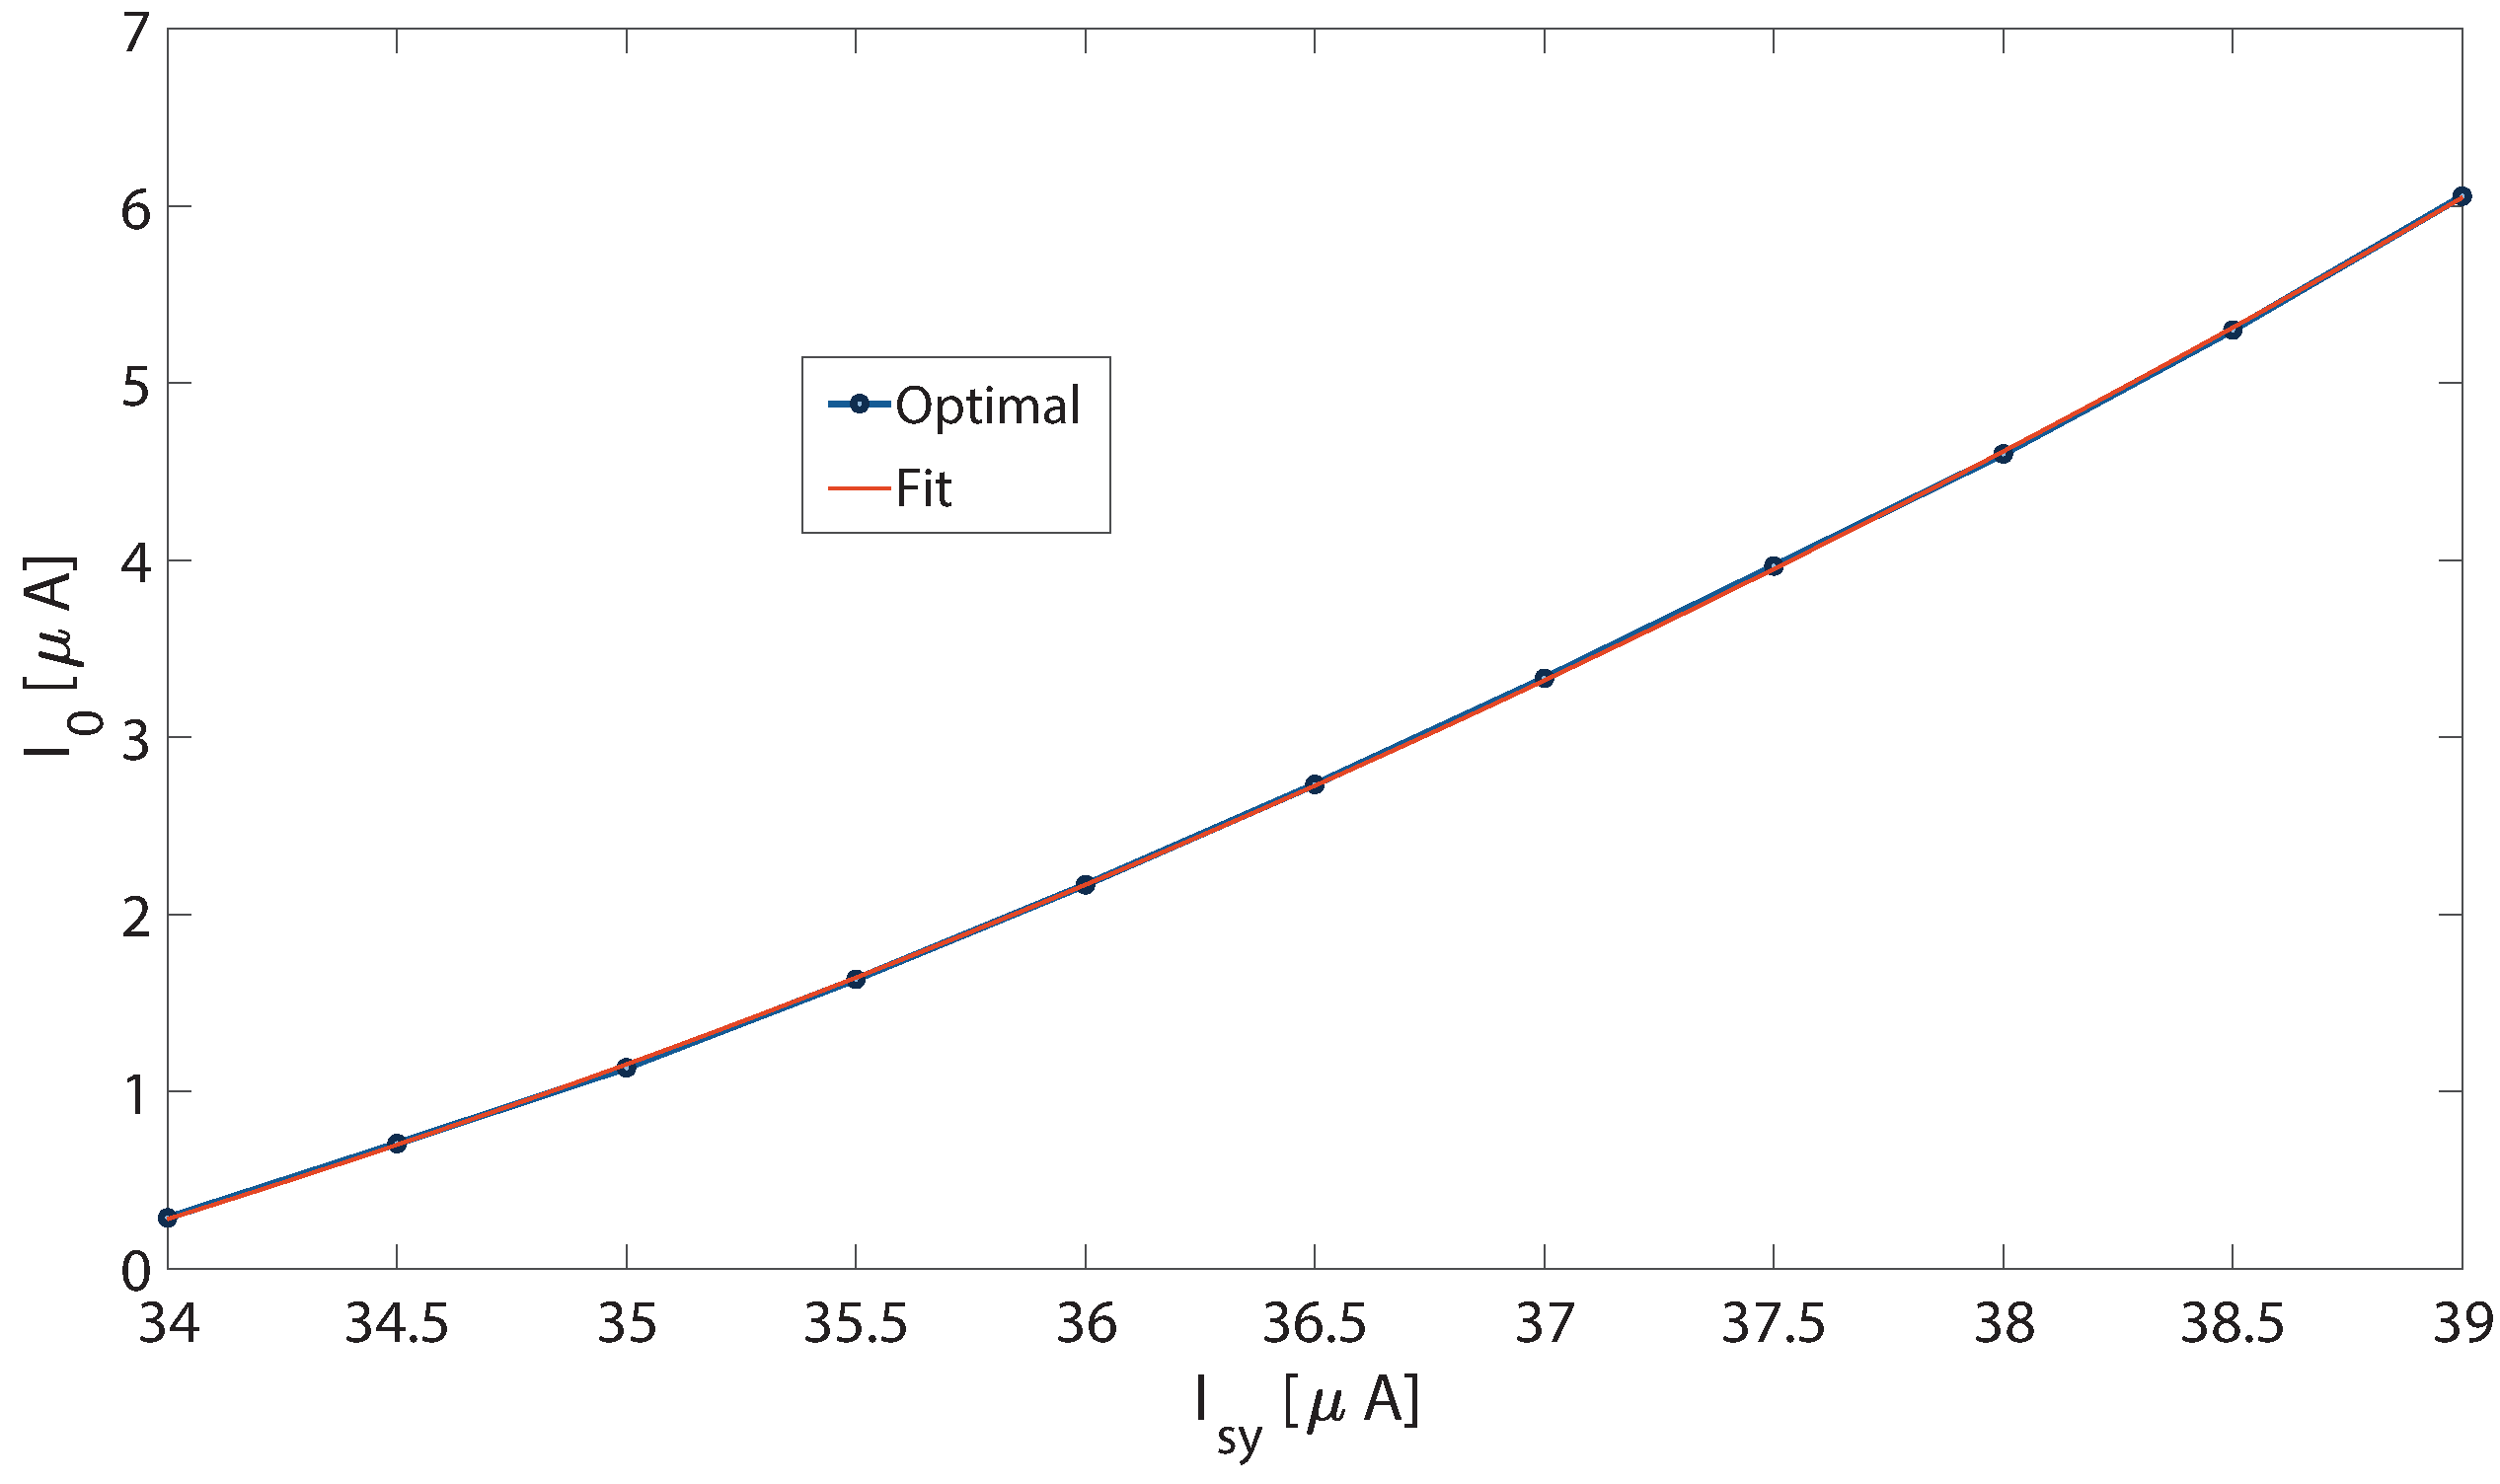
\includegraphics[width=17.2cm]{_I0_vs_Isy.pdf}
%\captionof{figure}{\label{fig:I0_vs_Isy}Optimized values of $I_0(I_{sy})$ and a polynomial fit.}
%\end{figure}
%We find the phenomenological functional form provides an excellent fit with
%\begin{equation}
%\label{eq:I0_vs_Isy}
%I_{0}\big(I_{sy}\big) = 0.06989 I_{sy}^2 - 3.948 I_{sy} + 53.73.
%\end{equation}
%Currents are in microamps. Equation \ref{eq:I0_vs_Isy} allows us to quickly calculate the amplitude of the post-synaptic response based on the value of the synaptic bias current, $I_{sy}$, at the time of input arrival. This is the synaptic weight.
%\begin{figure}[h!]
%\centering
%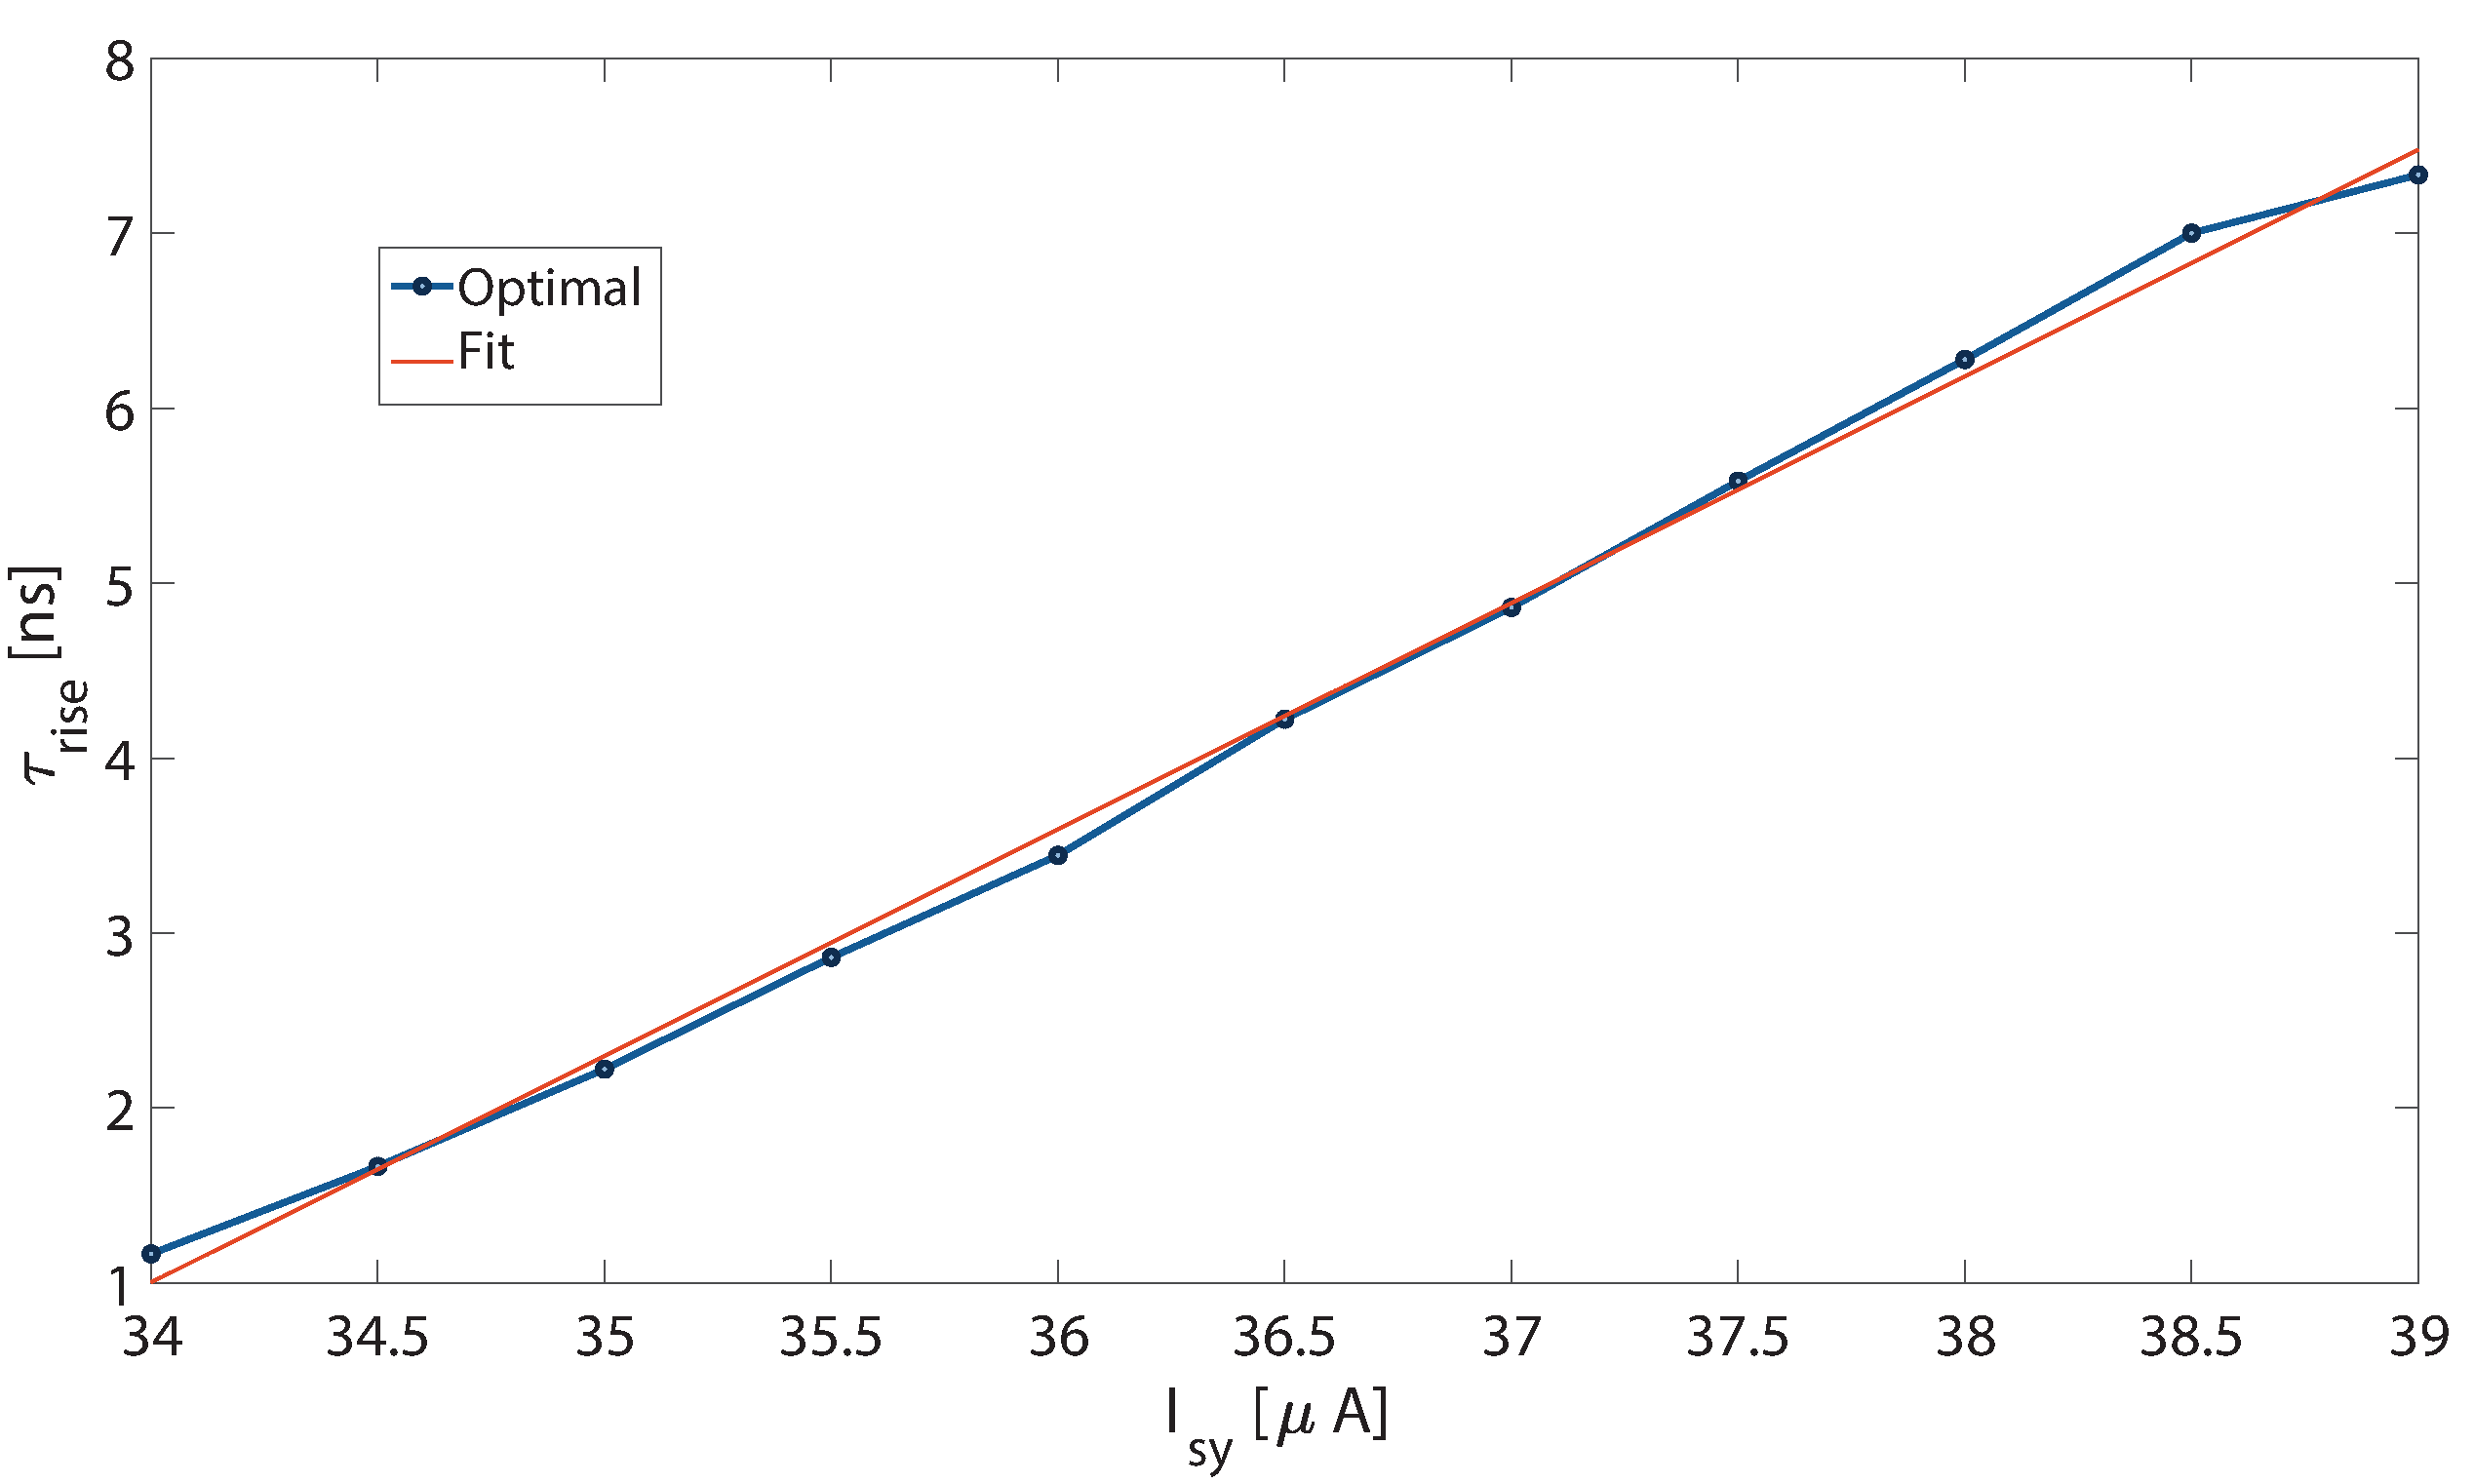
\includegraphics[width=17.2cm]{_tau_rise_vs_Isy.pdf}
%\captionof{figure}{\label{fig:tau_rise_vs_Isy}Optimized values of $\tau_+(I_{sy})$ and a linear fit.}
%\end{figure}
%
%Next we determine the time constant of the rising edge of the post-synaptic response, $\tau_{+}$. This is carried out with the same procedure as for $I_0(I_{sy})$, and the result is fit to a line. The data is shown in Fig.\,\ref{fig:tau_rise_vs_Isy}.
%We find the phenomenological functional form provides an excellent fit with
%\begin{equation}
%\label{eq:I0_vs_Isy}
%\tau_+\big(I_{sy}\big) =  1.294 I_{sy} - 43.01.
%\end{equation}
%With $I_{sy}$ in microamps, this fit provides $\tau_+$ in nanoseconds.
%
%%\begin{figure}[t!]
%%\centering
%%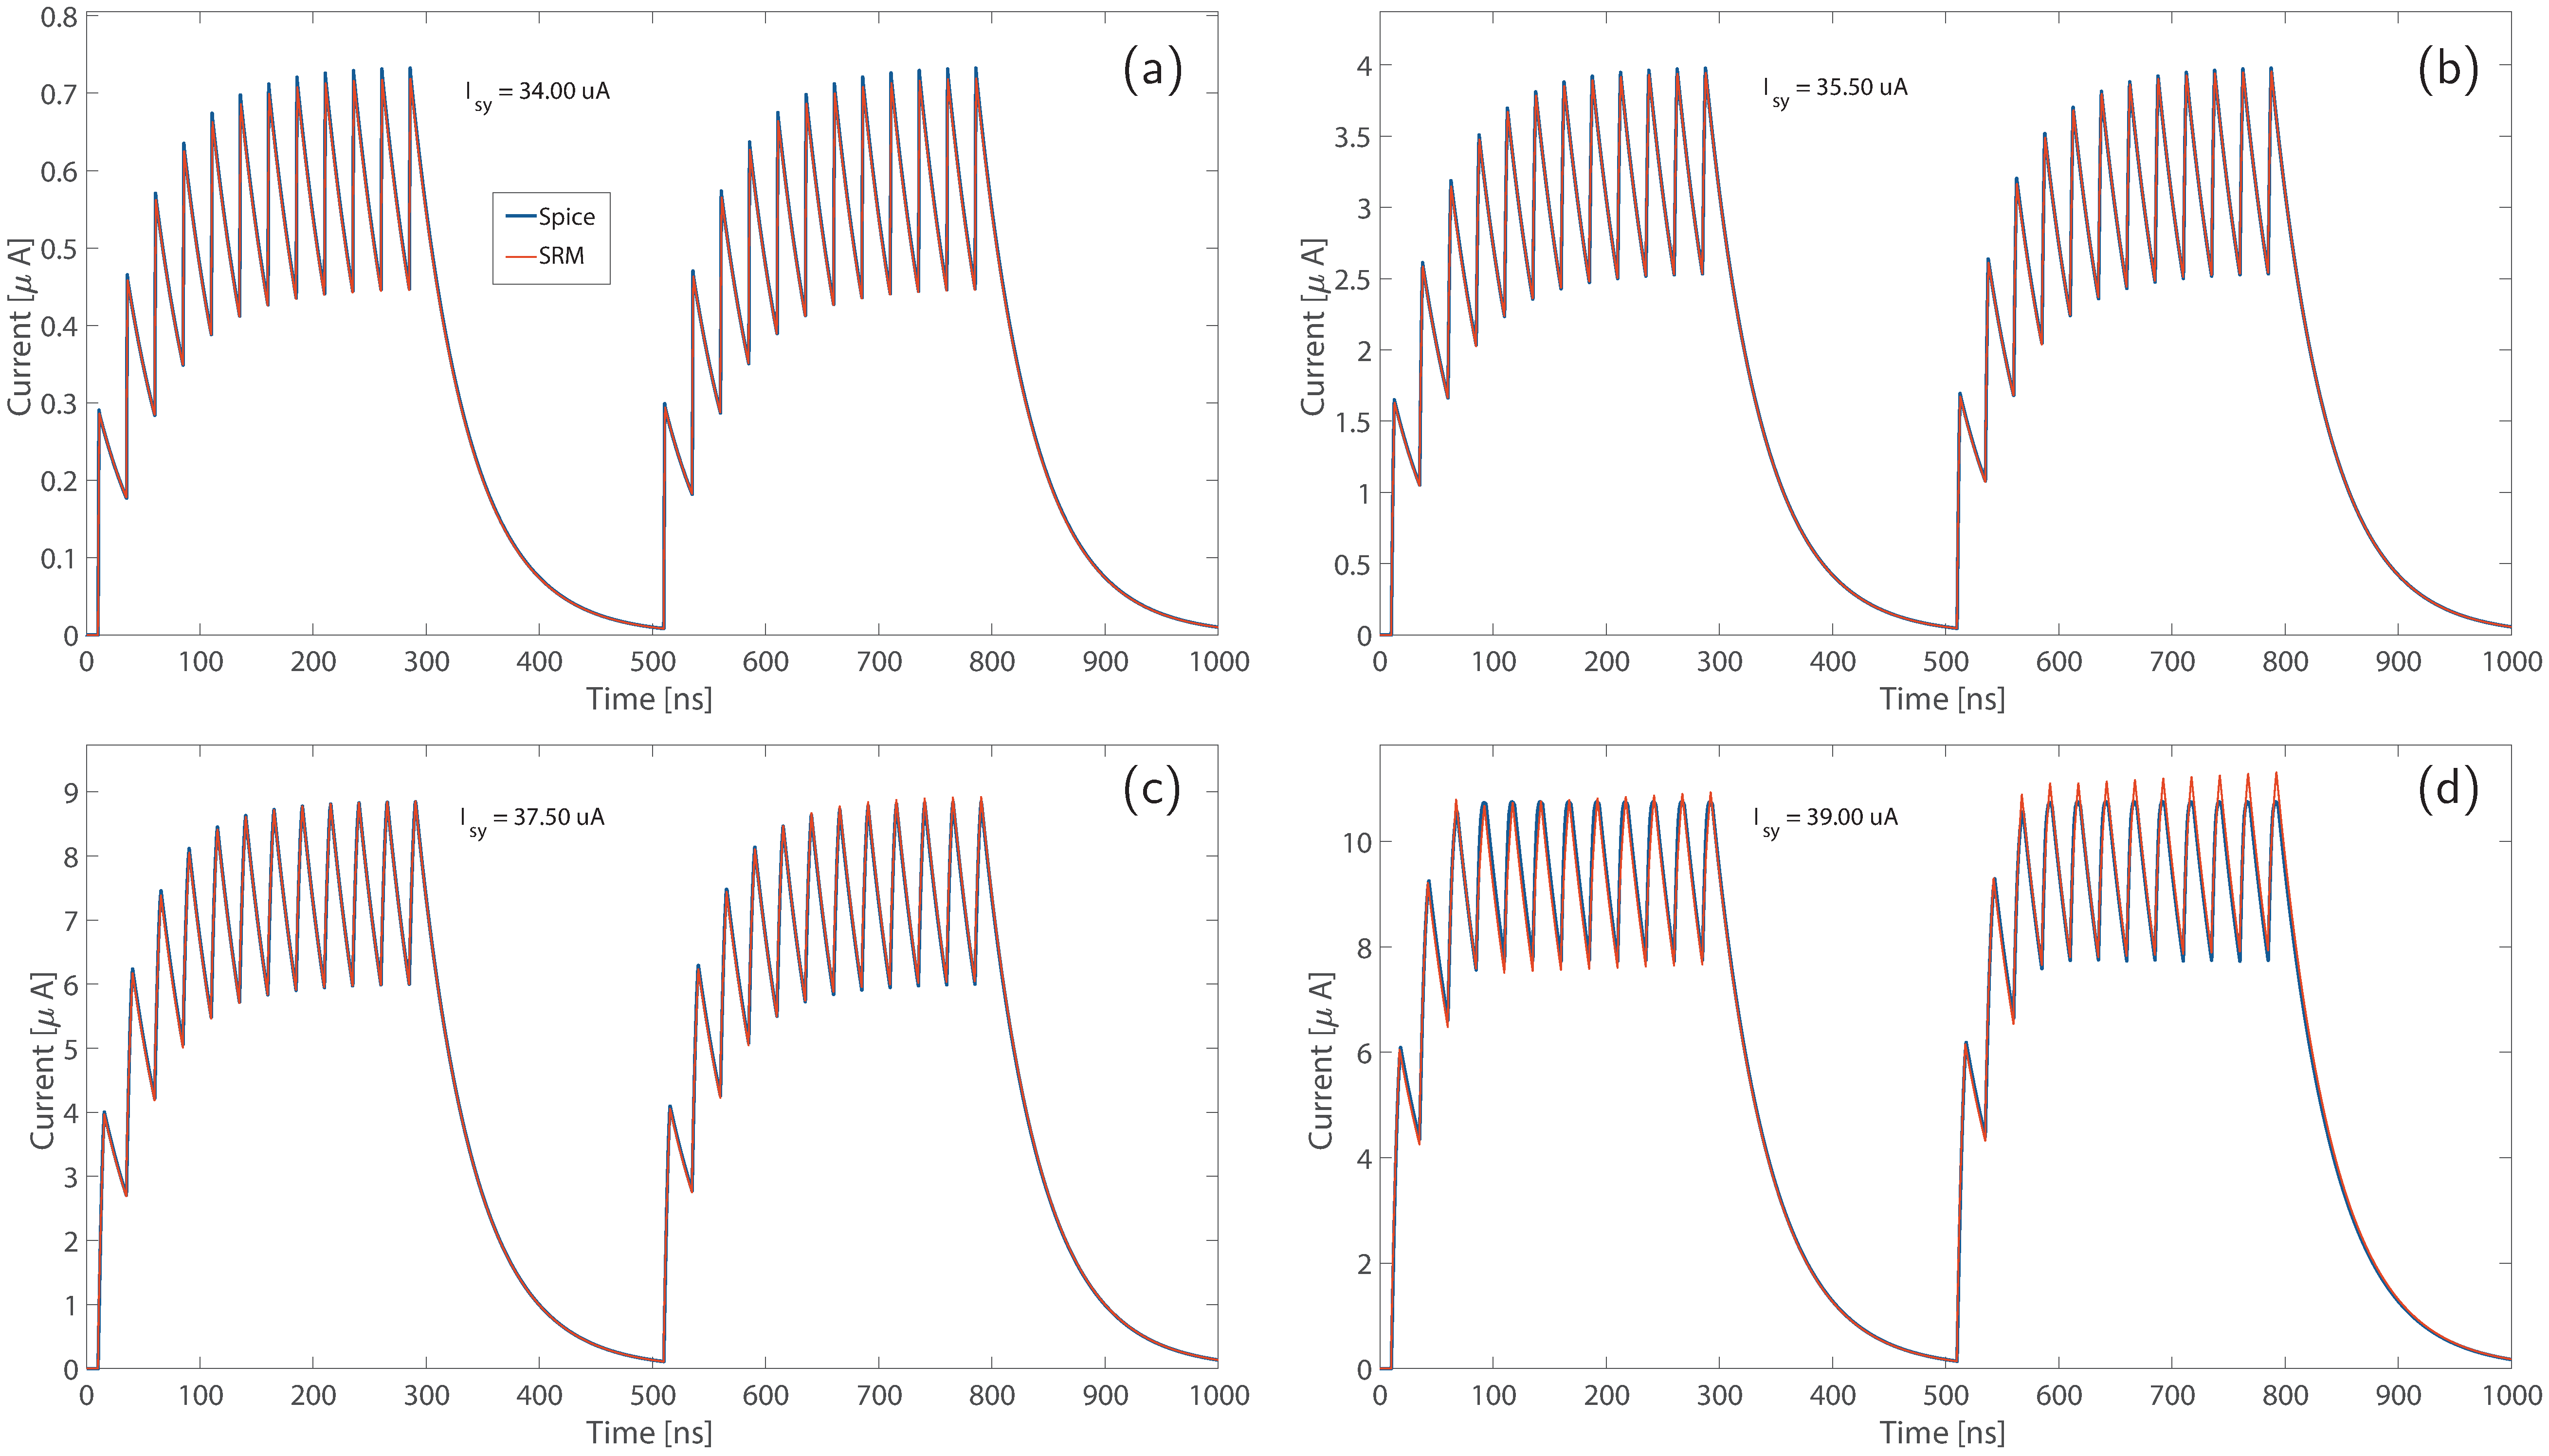
\includegraphics[width=17.2cm]{_time_traces__varying_Isy.pdf}
%%\captionof{figure}{\label{fig:time_traces__varying_Isy}Temporal traces for four values of $I_{sy}$. Blue traces are Spice and red are the model presented here. (a) $I_{sy} = 34$\,\textmu A. (b) $I_{sy} = 35.5$\,\textmu A. (c) $I_{sy} = 37.5$\,\textmu A. (d) $I_{sy} = 39$\,\textmu A. In these simulations, $L_{si} = 50$\,nH, $r_{si}=1\,\Omega$, and the input rate is 40\,MHz during the bursts. The model is not razor accurate, particularly not close to saturation, but I think it is good enough to do all the modeling in the near term for the projects discussed in Sec.\,\ref{sec:future_directions}.}
%%\end{figure}
%These values of the various parameters and fits specify the phenomenological spike response model. Now let's make sure the model works. Here we compare the model to temporal traces obtained from time-domain circuit simulations. Figure \ref{fig:time_traces__varying_Isy} shows temporal traces for an arbitrary input pulse sequence for four values of $I_{sy}$. Figure \ref{fig:error_vs_Isy} quantifies the error more systematically. The error is defined in Eq.\,\ref{eq:finding_gammas__error}.
%
%%\begin{figure}[t!]
%%\centering
%%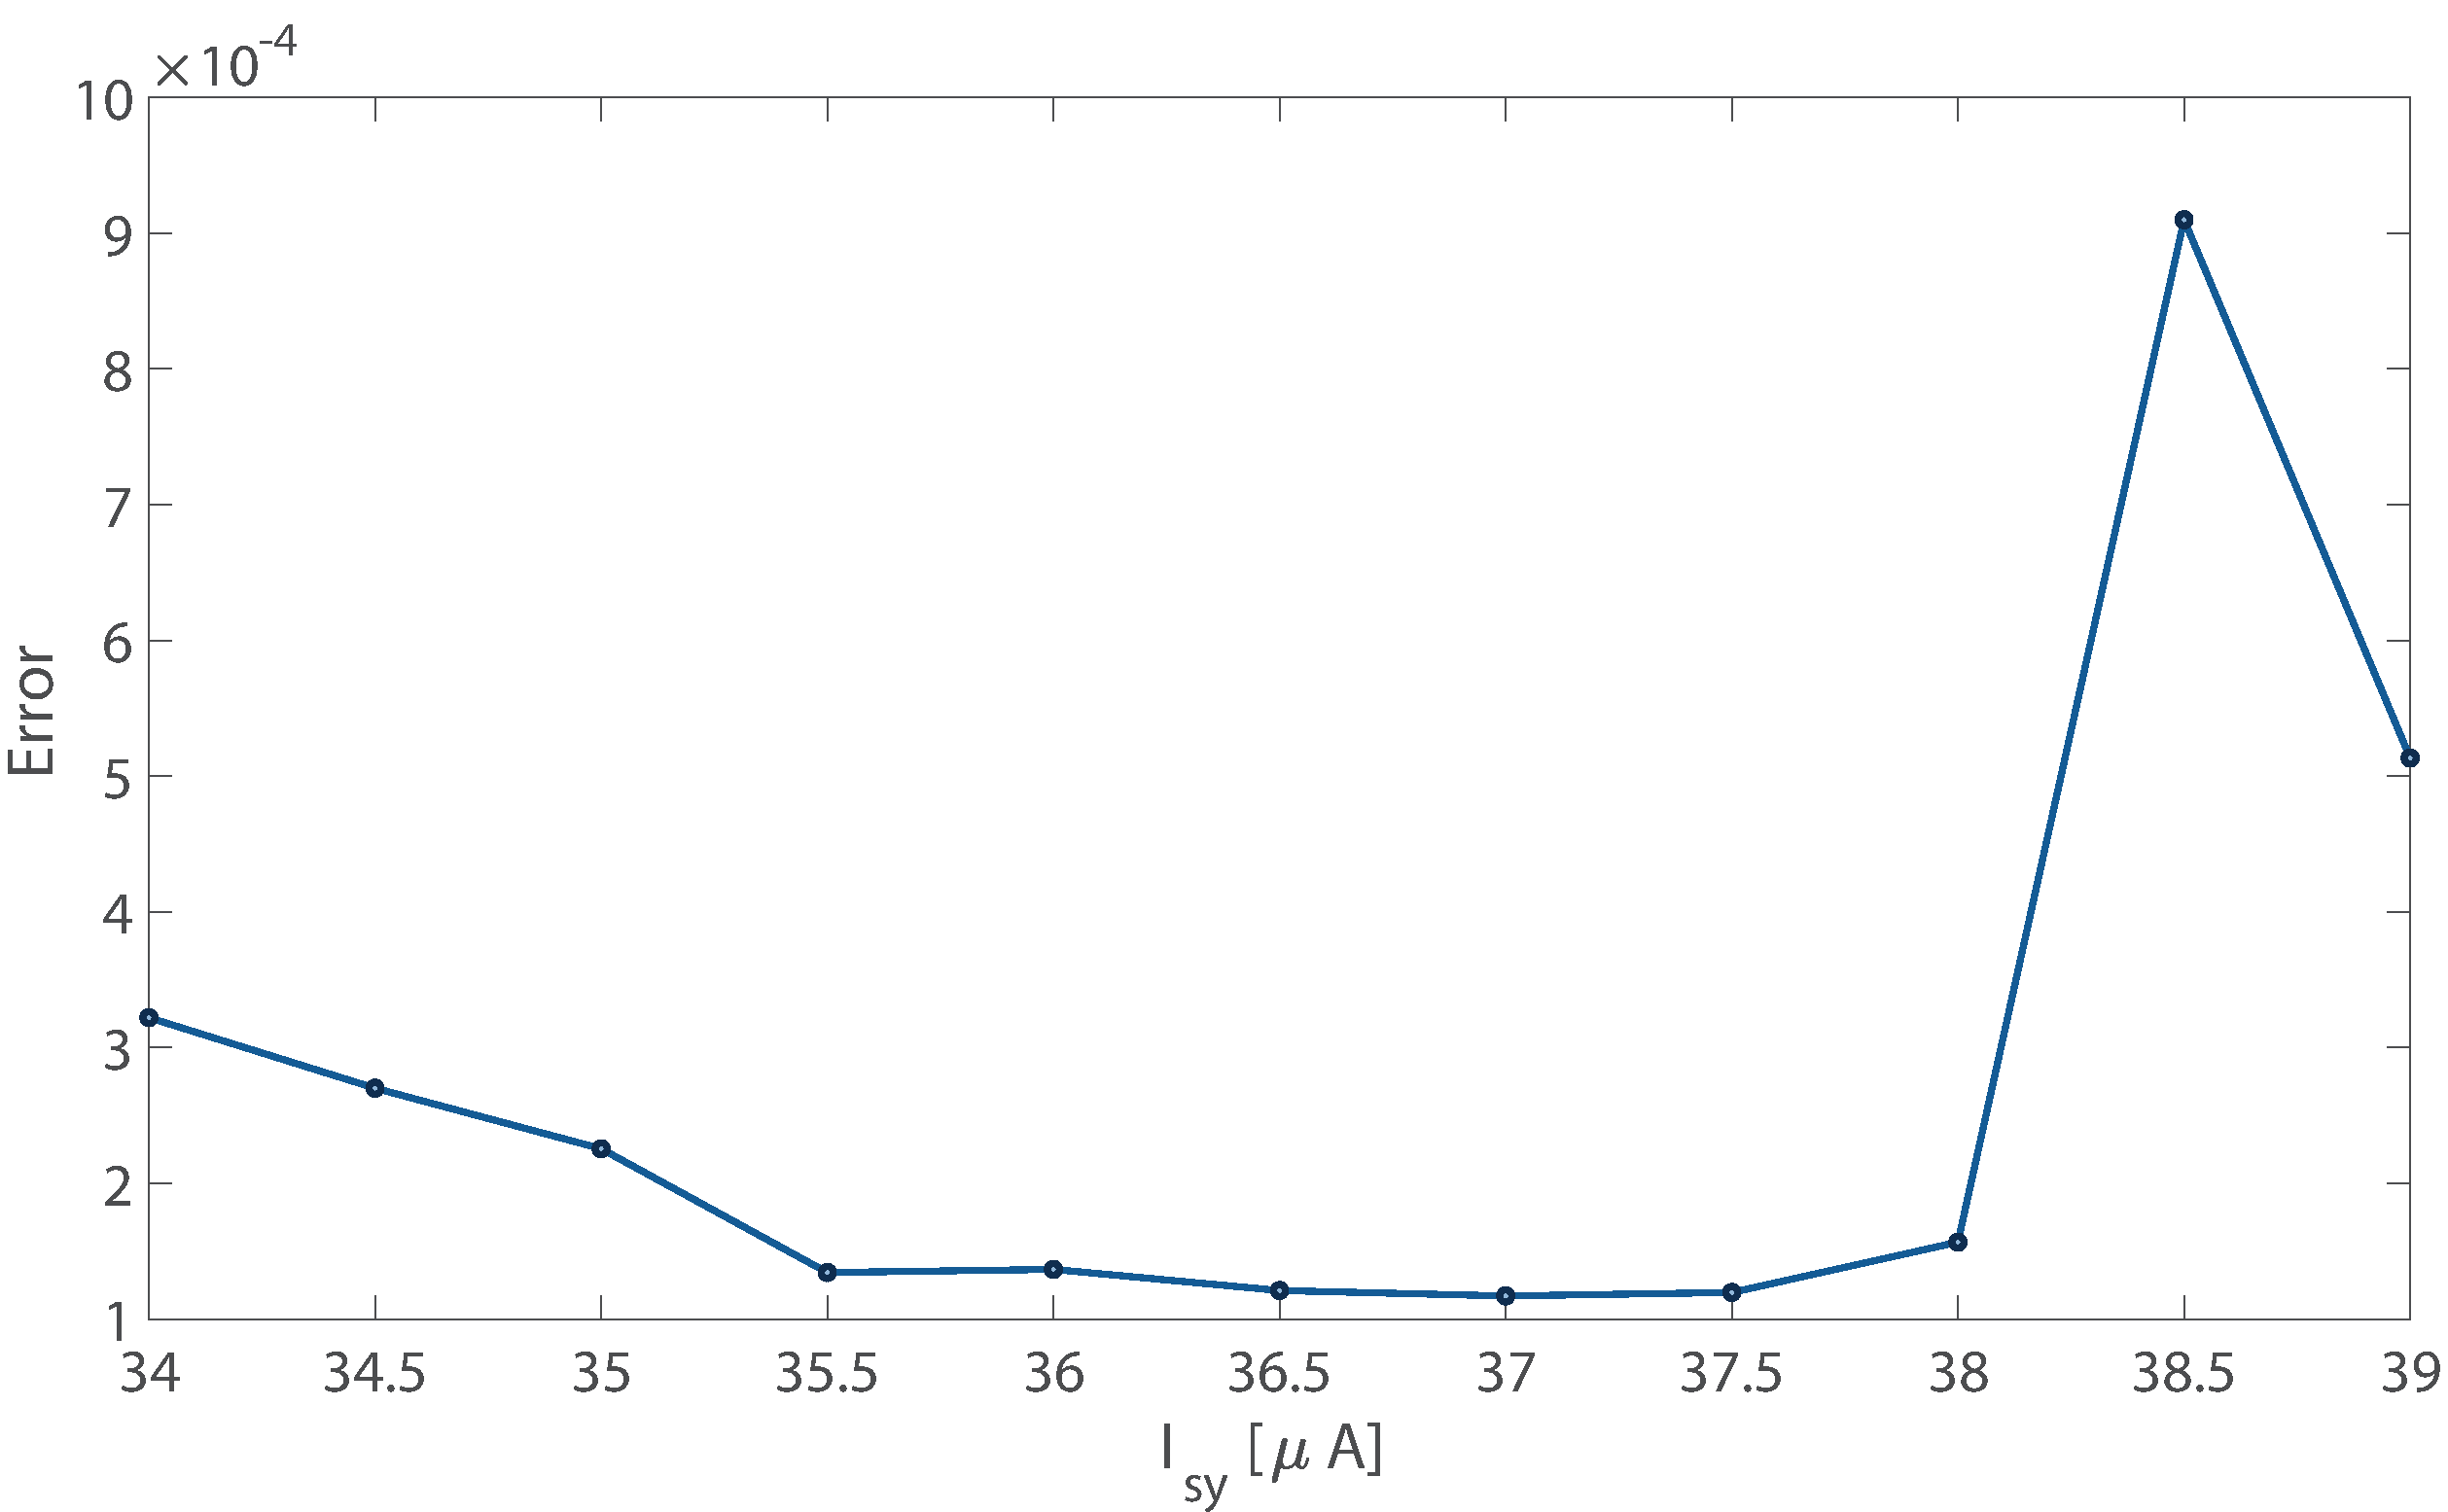
\includegraphics[width=17.2cm]{_error_vs_Isy.pdf}
%%\captionof{figure}{\label{fig:error_vs_Isy}Error versus $I_{sy}$. Good enough. $L_{si} = 50$\,nH, $r_{si}=1\,\Omega$, and the input rate is 40\,MHz during the bursts.}
%%\end{figure}
%
%%\begin{figure}[t!]
%%\centering
%%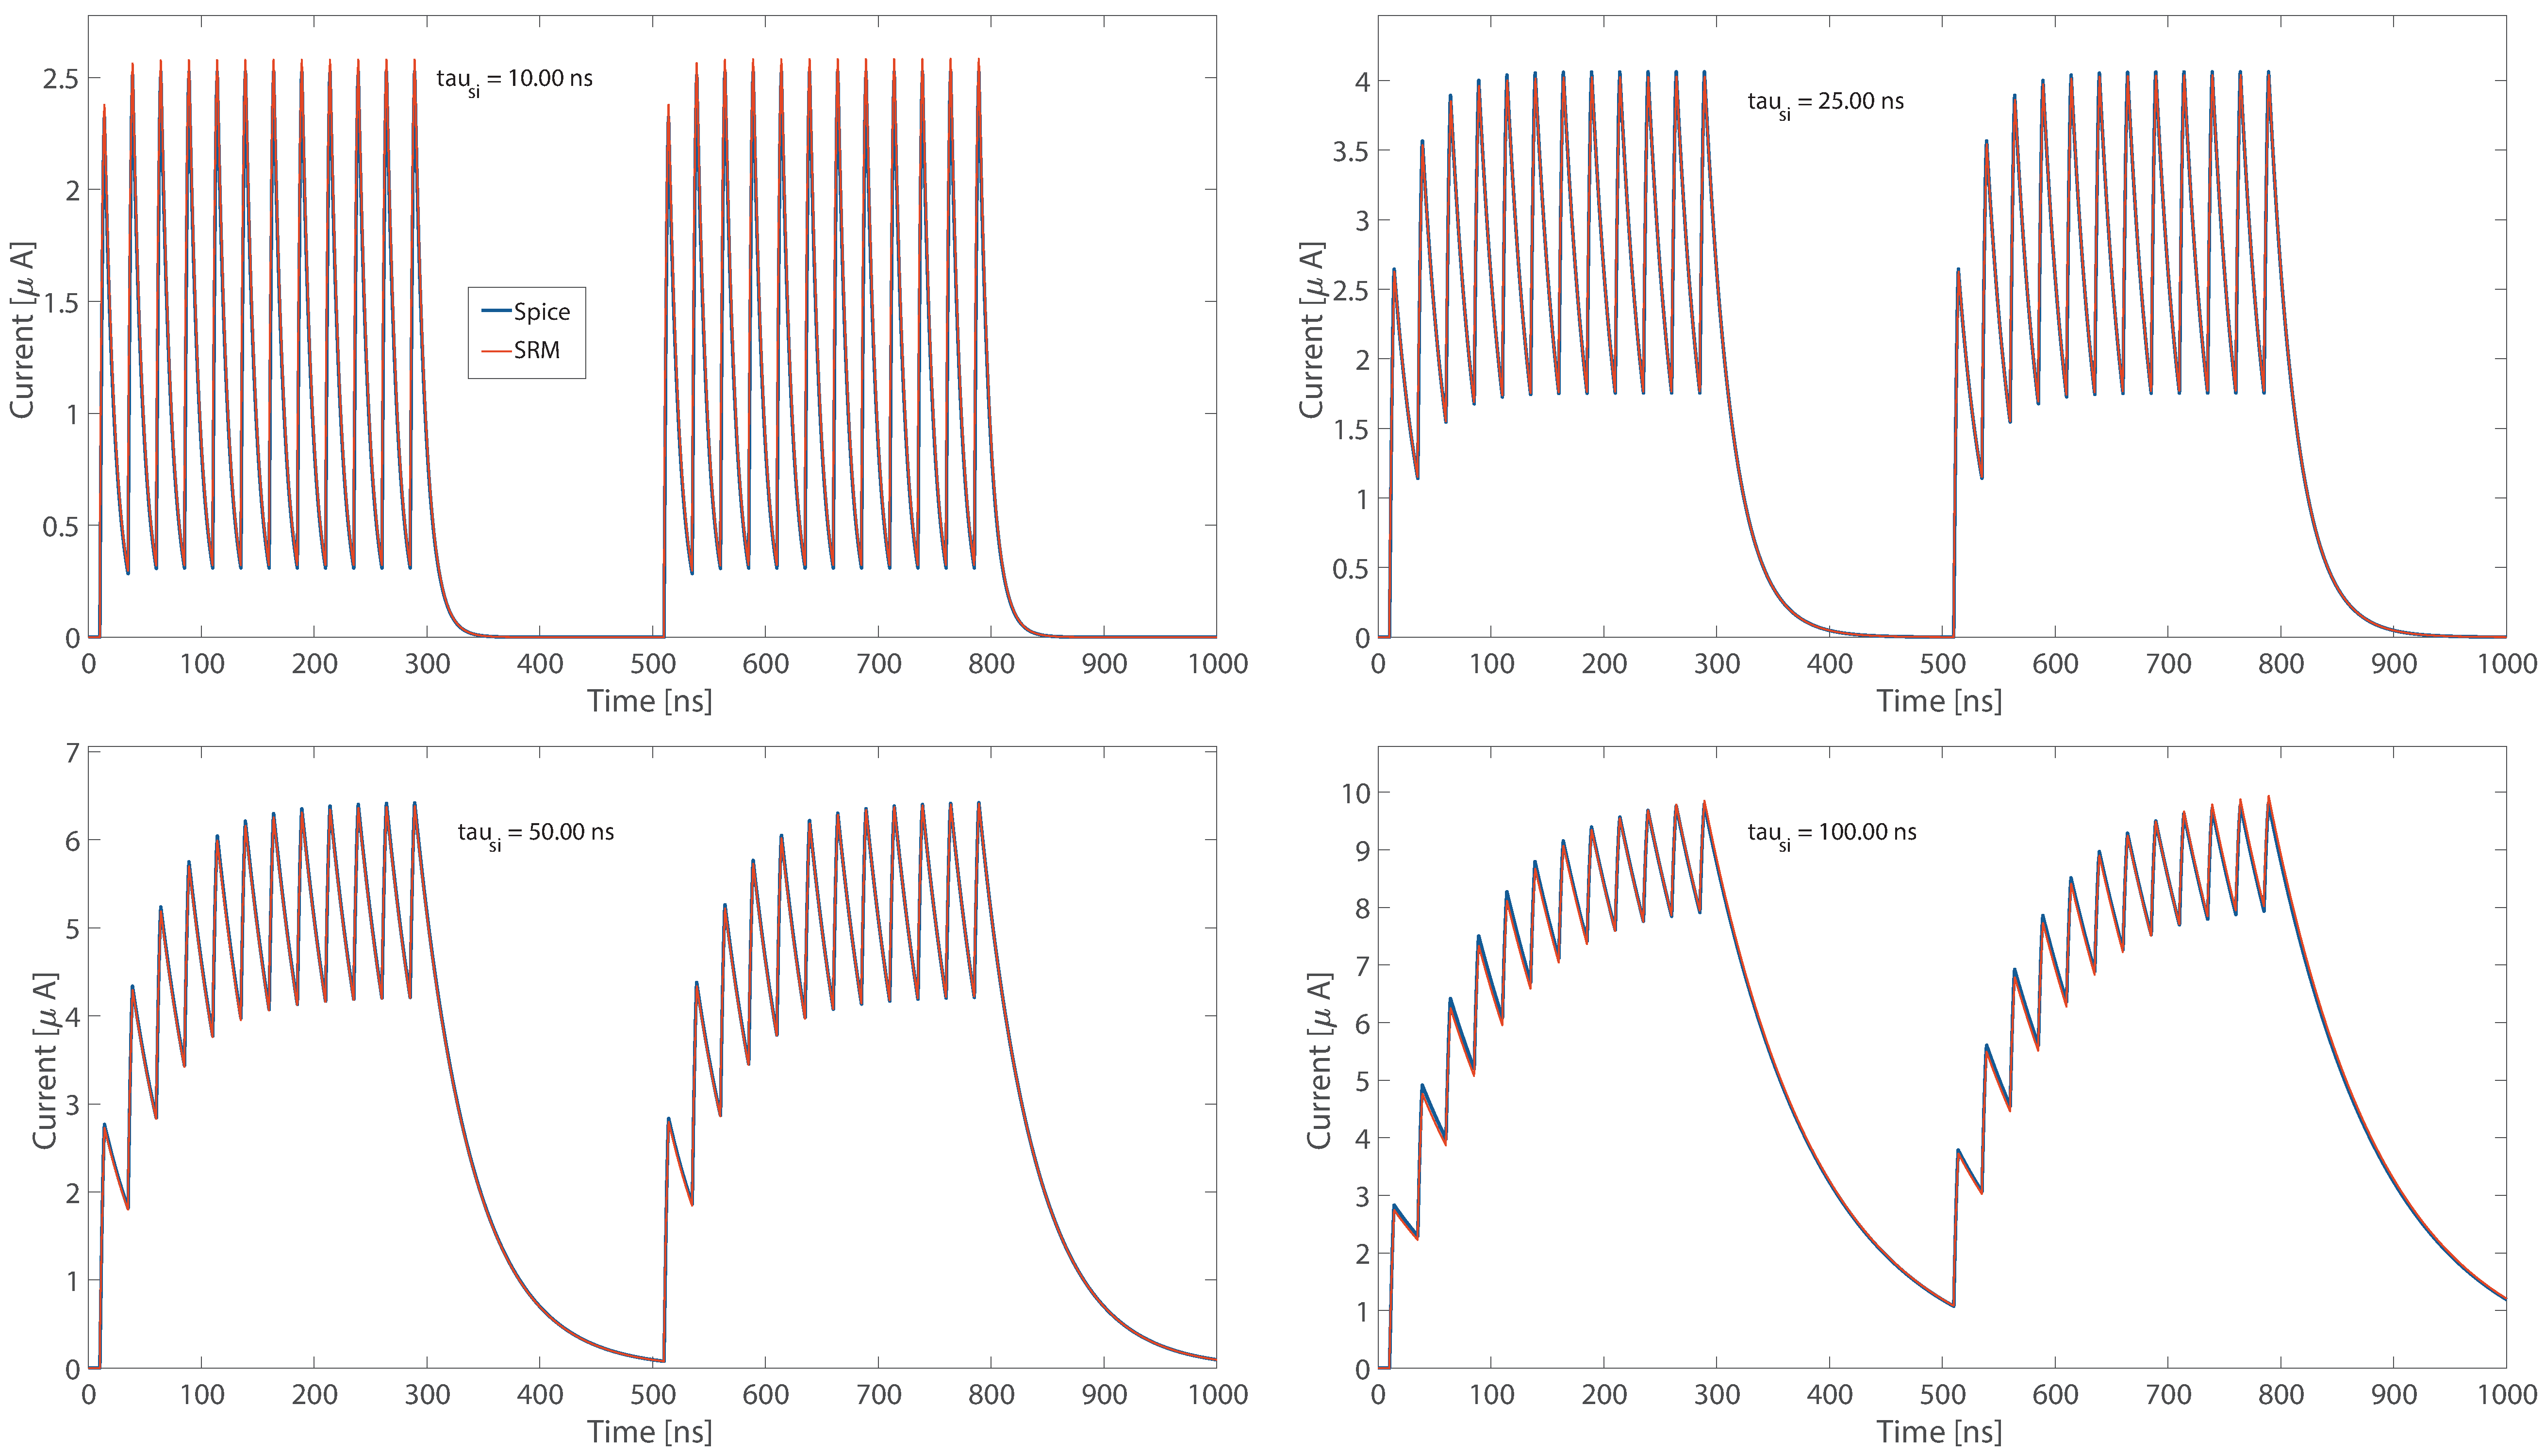
\includegraphics[width=17.2cm]{_time_traces__varying_tau_si.pdf}
%%\captionof{figure}{\label{fig:time_traces__varying_tau_si}Temporal traces for four values of $\tau_{si}$. Blue traces are Spice and red are the model presented here. (a) $\tau_{si} = 10$\,ns. (b) $\tau_{si} = 25$\,ns. (c) $\tau_{si} = 50$\,ns. (d) $\tau_{si} = 100$\,ns. In these simulations, $I_{sy} = 36.5$\,\textmu A, $L_{si} = 50$\,nH, $r_{si}$ is adjusted to achieve the value of $\tau_{si}$, and the input rate is 40\,MHz during the bursts.}
%%\end{figure}
%We also compare the model to circuit simulations for four values of $\tau_{si}$. These comparisons are shown in Fig.\,\ref{fig:time_traces__varying_tau_si}, and the error is quantified systematically in Fig.\,\ref{fig:error_vs_tau_si}. Note that for very fast values of $\tau_{si}$, the value of $I_0$ should be adjusted. This is of minor importance and will usually not matter, but I don't want to forget about it, so more information is in Appendix \ref{apx:dependence_of_I0_on_tau_si}.
%
%%\begin{figure}[t!]
%%\centering
%%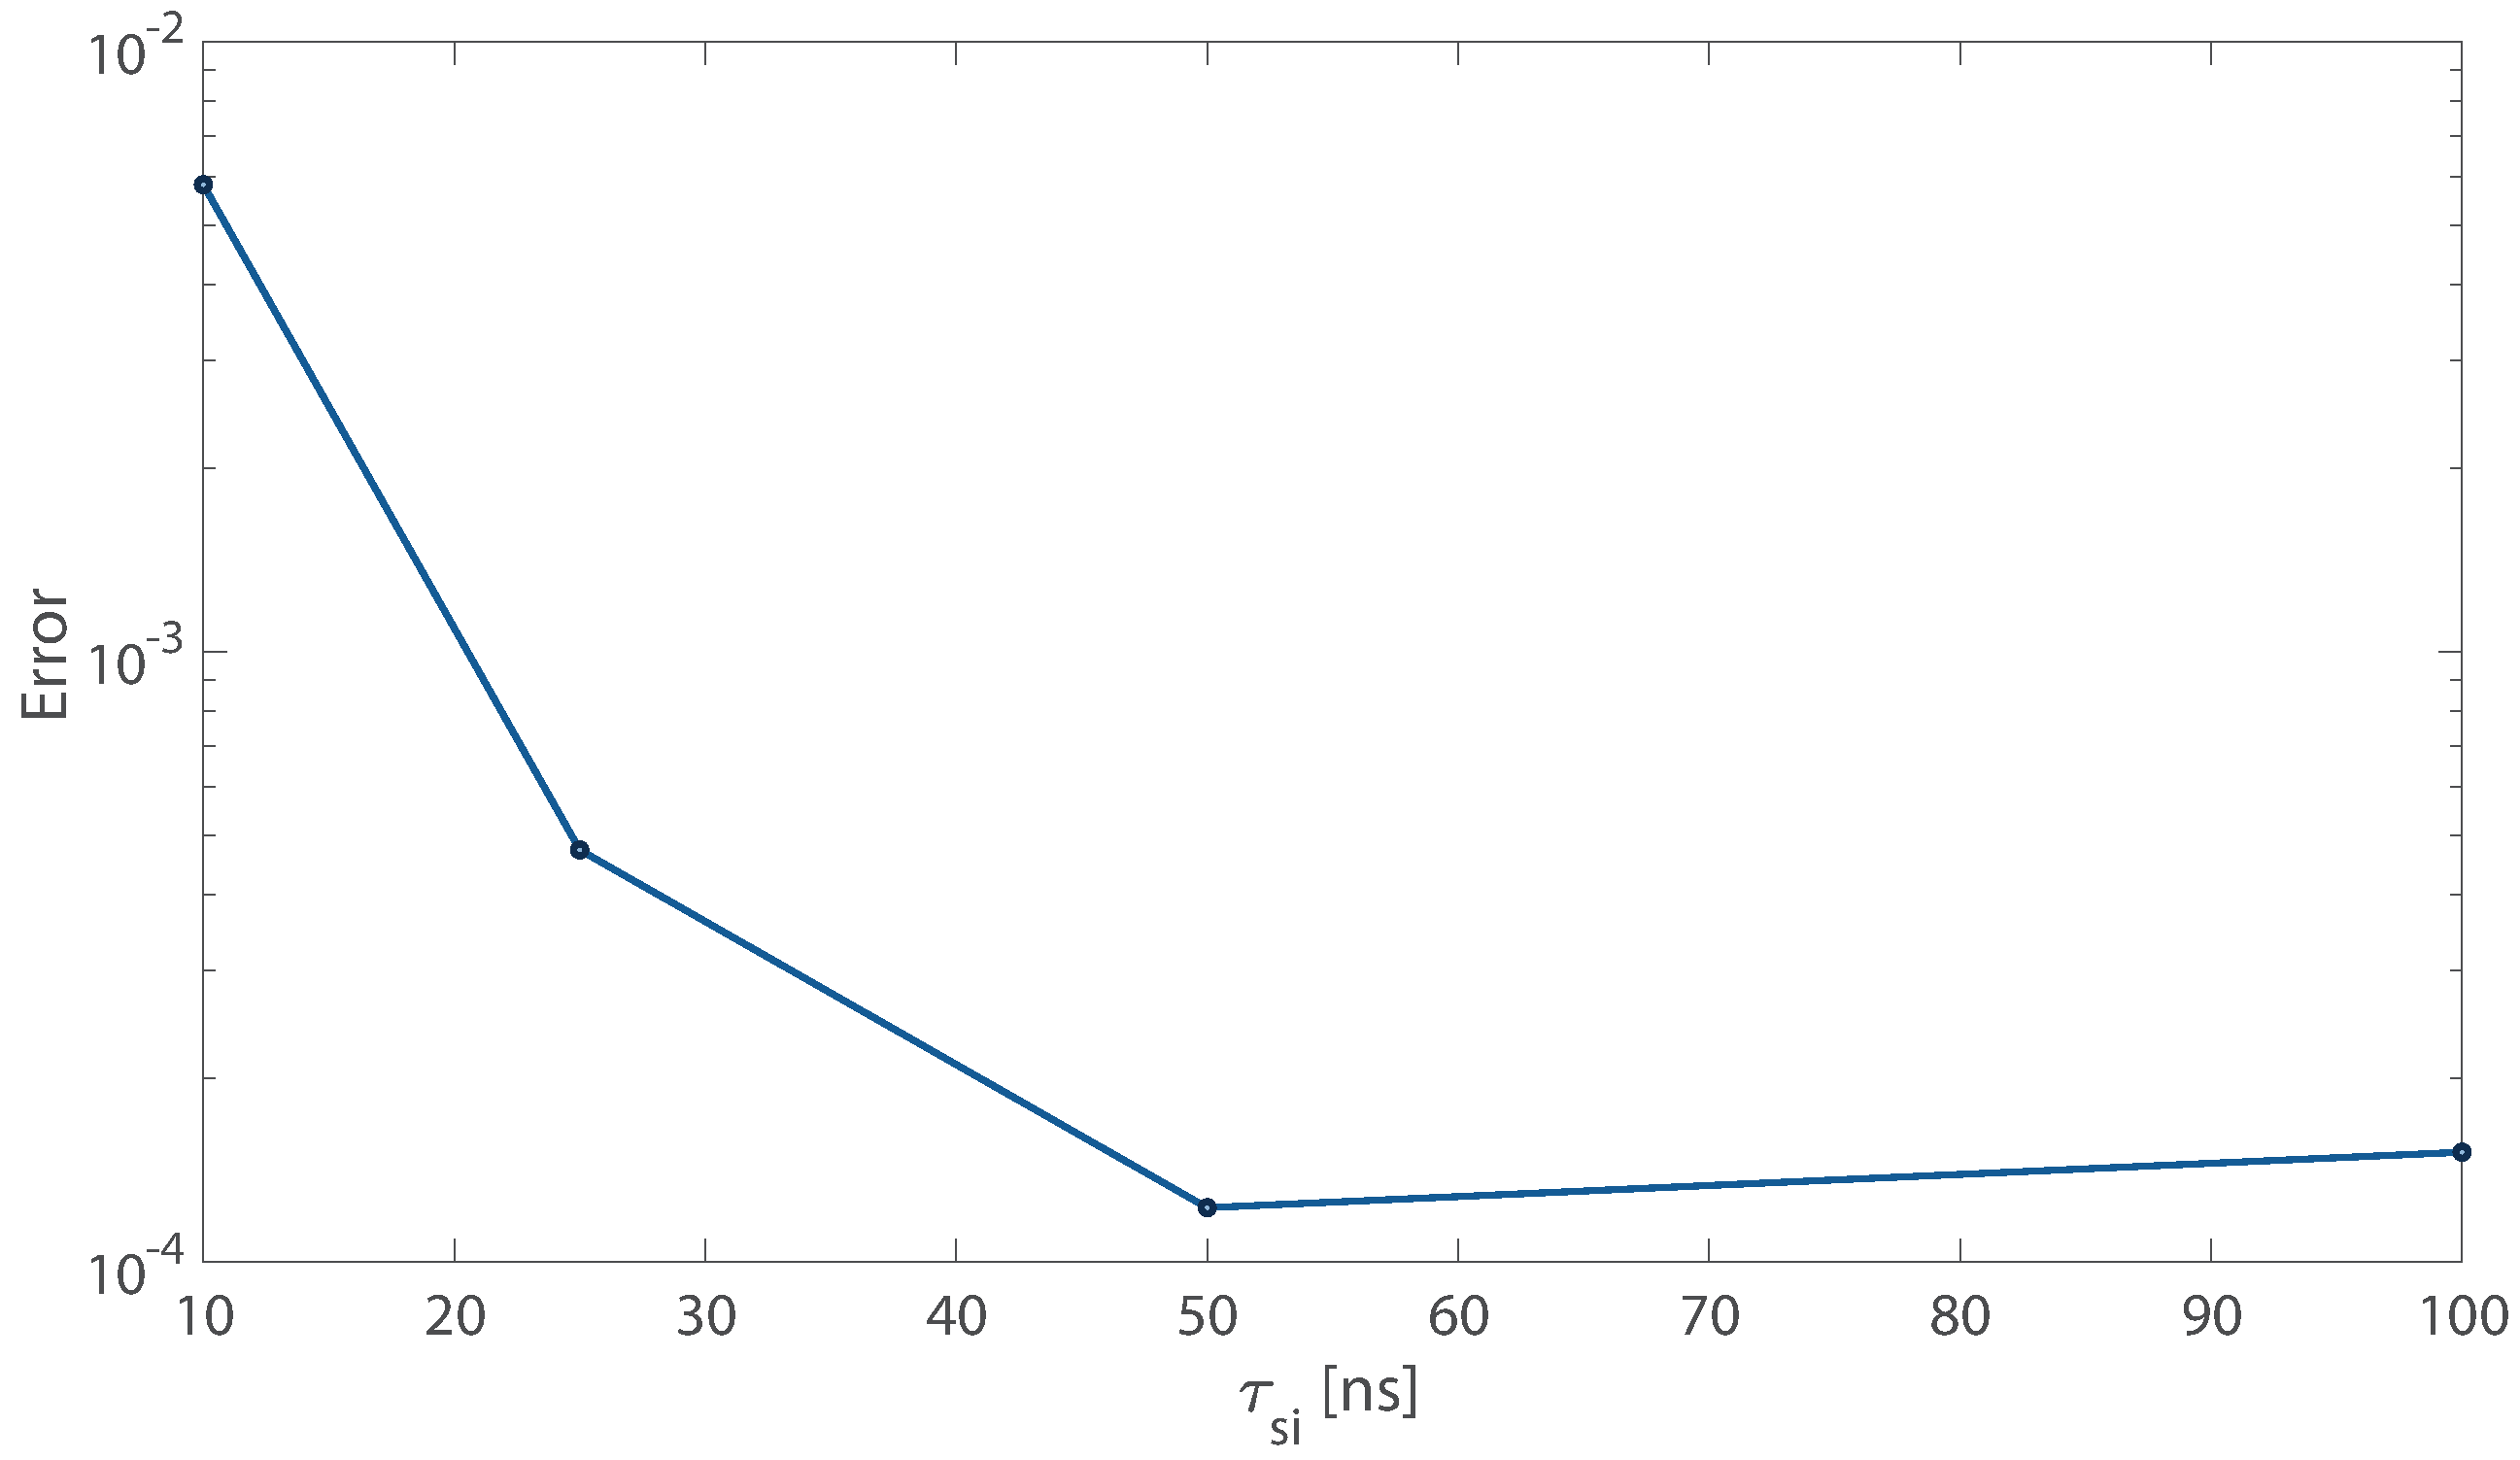
\includegraphics[width=17.2cm]{_error_vs_tau_si.pdf}
%%\captionof{figure}{\label{fig:error_vs_tau_si}Error versus $\tau_{si}$. $I_{sy} = 36.5$\,\textmu A, $L_{si} = 50$\,nH, $r_{si}$ is varied to achieve $\tau_{si}$, and the input rate is 40\,MHz during the bursts. The error is worse for SI loops with fast leak rates, but it is still acceptable for the present purposes.}
%%\end{figure}
%
%%\begin{figure}[t!]
%%\centering
%%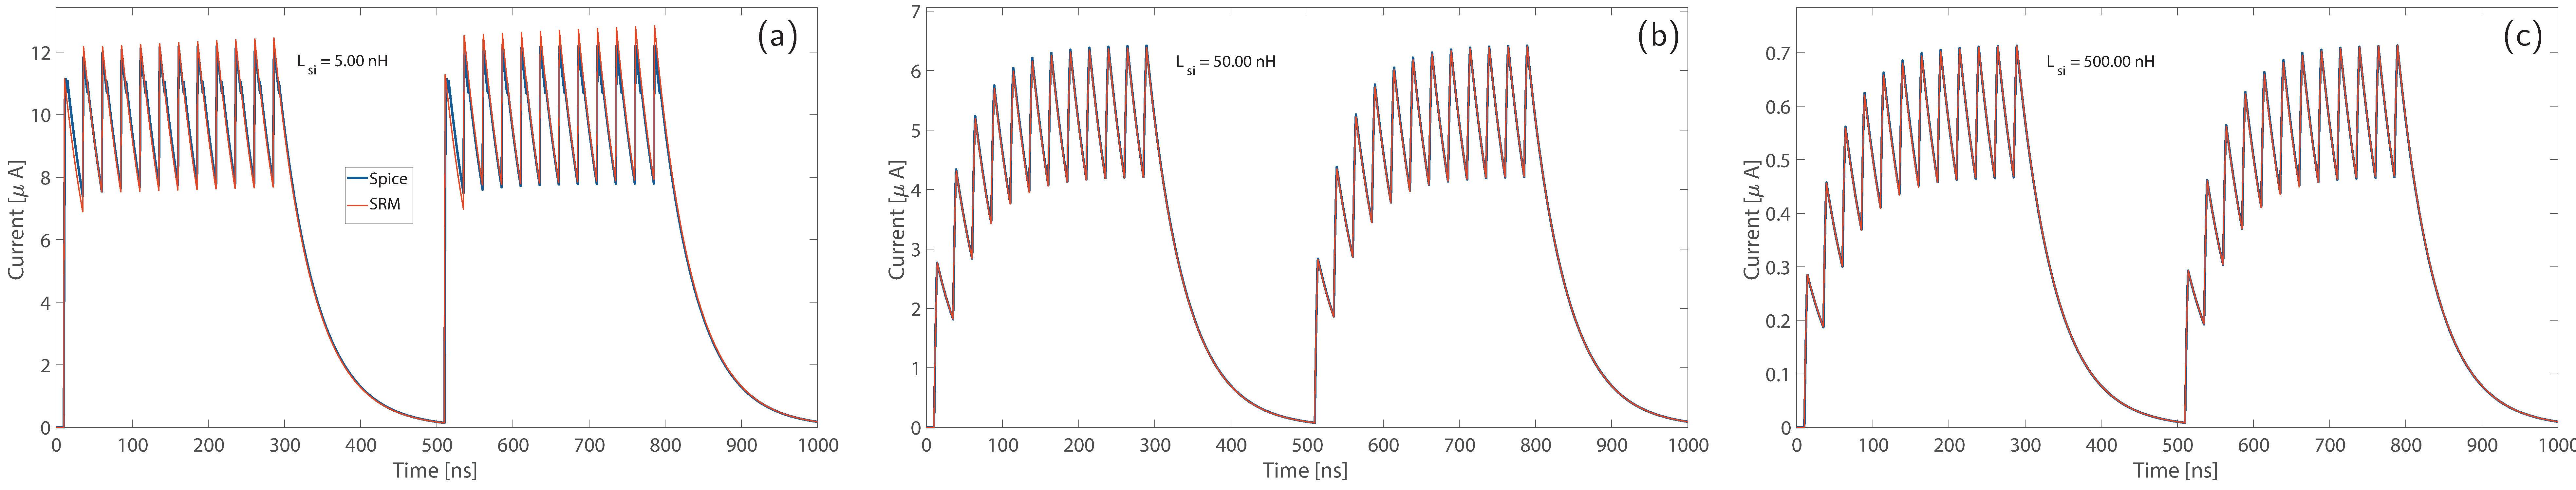
\includegraphics[width=17.2cm]{_time_traces__varying_L_si.pdf}
%%\captionof{figure}{\label{fig:time_traces__varying_L_si}Temporal traces for three values of $L_{si}$. Blue traces are Spice and red are the model presented here. (a) $L_{si} = 5$\,nH. (b) $L_{si} = 50$\,nH. (c) $L_{si} = 500$\,nH. In these simulations, $I_{sy} = 36.5$\,\textmu A, $r_{si}$ is adjusted to maintain $\tau_{si} = 50$\,ns, and the input rate is 40\,MHz during the bursts.}
%%\end{figure}
%Finally, we also check to make sure the model works across a broad range of SI loop storage sizes, quantified by $\beta_L$. These comparisons are shown in Fig.\,\ref{fig:time_traces__varying_L_si}. Again, agreement is satisfactory.
%
%\section{\label{sec:neurons}Phenomenological Model of Point Neurons}
%We have a closed-form expression (Eqs.\,\ref{eq:I_si} and \ref{eq:I_si__prefactor}) for the response of a synapse to a spike train represented by a list of input spike times $\bar{t}$. In the case of a point neuron, the response from all input synapses are weighted and summed. In loop neurons, the weights at this stage of summation are due to mutual inductors, so we write the current in the neuronal receiving (NR) loop as
%\begin{equation}
%\label{eq:I_nr}
%I^{nr}(t) = \sum_i m_i I_i^{si}(\bar{t}_i;t).
%\end{equation}
%Here $m_i$ is a fixed weight due to mutual induction. Plastic synaptic weights are discussed in Sec.\,\ref{sec:synaptic_plasticity}. 
%
%The neuron cell body has a threshold set by the critical current of the neuronal firing junction. When $I^{nr}(t) = I^{nr}_{th}$ and $\frac{dI^{nr}(t)}{dt} > 0$, $J_{nr}$ is driven to produce fluxons. In hardware, this results in triggering the hTron and the LED. This is a spike event. That device dynamics does not concern us here. We assume this process is fast relative to interspike intervals. We also assume activation of the hTron also drives a DCSFQ circuit that adds a fluxon to the refractory suppression (RS) loop. This refractory feedback adds a current to the NR loop of exactly the same form as the post-synaptic current, except this suppression current opposes the current added to the NR loop by all the excitatory synapses, thus driving the neuron below threshold. The refractory period depends on the amplitude of this current as well as the leak rate of the RS loop.
%
%Thus, refraction simply adds another term to the sum in Eq.\,\ref{eq:I_nr}, so we write the current in the neuronal receiving loop of neuron $j$ as
%\begin{equation}
%\label{eq:I_nr__with_refraction}
%I_i^{nr}(t) = m_i^{rs}I^{rs}(\bar{t}_i;t)+\sum_i m_{ij} I_j^{si}(\bar{t}_j;t).
%\end{equation}
%When the full form of $I^{si}$ (Eq.\,\ref{eq:I_si}) is inserted into Eq.\,\ref{eq:I_nr__with_refraction}, we see Eq.\,\ref{eq:I_nr__with_refraction} has the form of the SRM model, Eq.\,\ref{eq:spike_response_model}.
%
%To use the model of Eq.\,\ref{eq:I_nr__with_refraction} to simulate networks of loop neurons, one need not solve any ODEs, but I think it is still necessary to step through time on a fine mesh because one does not know the lists of spike times in advance. I think numerically one steps through the synaptic and neuronal equations and checks every neuron for the threshold condition at each time step. One of the primary reasons for producing this document is to solicit input as to how to best model these systems numerically.
%
%\section{\label{sec:subthreshold_oscillations}Subthreshold Membrane Oscillations}
%We have discussed a synaptic response that grows rapidly following a synaptic firing event and then decays exponentially in time. In biological neurons, a additional synaptic response occurs wherein the response to synaptic activity is an underdamped oscillatory function. Such a response leads to subthreshold membrane oscillations in the target neuron. There is substantial neuroscientific evidence that such oscillations are a means by which neurons can synchronize their activity. The synapses responsible for oscillatory responses are distinct from synapses with post-synaptic potential that decays without oscillations. If multiple neurons receive synapses from another neuron that induces subthreshold membrane oscillations can cause the ensemble of neurons to oscillate at the same frequency with the same phase. Subsequently, this ensemble is likely to produce activity at the peak of the oscillations, as the neurons will effectively experience reduced thresholds at the synchronized times, and other inputs from elsewhere in the network may then be sufficient to evoke action potentials.
%
%In loop neurons, subthreshold membrane oscillations can be evoked in either dendrites or the neuron cell body when the usual inductive SI loop is augmented with a capacitance. For this to be useful, the oscillation frequency of the LC circuits [$(LC)^{-1/2}$] must be on the order of the frequency at which we expect network oscillations to occur. For loop neurons, this time scale is set by the recovery time of the photon detectors at the synaptic receivers as well as the recovery time of the amplifier chain responsible for light production, and it leads to peak spike frequencies around 100\,MHz. I think of frequencies close to 100\,MHz as the $\gamma$ oscillations of the system, but we would also like to induce synchronized activity on slower time scales analogous to brain-wide $\theta$ oscillations, which would be at 10\,MHz or even 1\,MHz. While this is typically difficult to achieve with normal metals in compact circuits, we can obtain a broad range of time constants with superconducting circuits. This is a major strength of using superconductors. Just as the $L/r$ time constants discussed above can cover a broad range due to the ability to achieve large $L$ and small $r$ as well as small $L$ and large $r$, here we can achieve long $LC$ time constants using capacitors of modest capacitance and inductors of large inductance. Capacitors are often huge, occupying hundreds of \textmu m$^2$ for a few hundred femtofarads. This is okay if you have one per neuron, but not one per synapse. With normal metals, it is impossible to achieve large inductance without also incurring large resistance, so $LC$ oscillators are not typically utilized in integrated microelectronics. But nature gives us superconducting materials with very high kinetic inductance, so we can make very large inductors that are extremely useful in achieving the basic parameters of the circuits discussed here. With a compact wire meander in series with a capacitor, we can achieve subthreshold membrane oscillations down to kilohertz and up to gigahertz range, covering the $\theta$ and $\gamma$ frequencies of interest.
%
%In the model under consideration, this is implemented straightforwardly by multiplying each term in Eq.\,\ref{eq:I_si} by $\mathrm{cos}[\omega_{LC} (t-t_q)]$ to achieve a damped, oscillatory post-synaptic potential. As discussed above, the primary function of such a synapse is to induce synchronized oscillations. Thus, such a circuit is most advantageous if multiple neurons can have their membrane potential modulated by this exact same post-synaptic potential. In biology, this would be difficult. In superconducting hardware, it is straightforward. A single synapse with an oscillatory integration loop (one central capacitor and long inductor wire) can be directly coupled to the cell bodies of multiple neurons with the usual mutual inductors. In this way, many neurons can be driven with exactly the same subthreshold membrane oscillations, thereby ensuring phase coherence.
%
%\section{\label{sec:synaptic_plasticity}Treatment of Synaptic Plasticity}
%Another important phenomenon that can be captured in this model is synaptic plasticity. Each synapse has a synaptic bias current, $I_{sy}$, that determines the synaptic weight. When numerically implementing this model, one must keep track of the state of each synapse ($I_{si}(t)$), but one can also investigate plasticity mechanisms by keeping track of each synaptic weight ($I_{sy}(t)$). Essentially any learning rule one can think of can be implemented to update $I_{sy}$ based on correlated activity between synapses and neurons for various forms of spike-timing-dependent plasticity. In loop neurons, $I_{sy}(t)$ is determined by the state of flux in a superconducting storage loop, just like $I_{si}(t)$, so one can utilize nearly identical equations to model activity-dependent modifications to $I_{sy}(t)$. One difference is that we assume $I_{sy}(t)$ has no leak (or at least very large $L/r$), but the model can handle this just fine due to the nature of the prefactor term, Eq.\,\ref{eq:I_si__prefactor}, that handles loop saturation. Another difference is that update of the state of $I_{sy}(t)$ usually depends on correlated activity between two neurons, whereas Eq.\,\ref{eq:I_si} only takes a single spike-time vector ($\bar{t}$) as input. In this way, synaptic update is more like a two-synapses dendrite that responds based on coincidences. This will be explored in more detail in Sec.\,\ref{sec:dendrites}. While I have explored synaptic plasticity in these circuits based on circuit models \cite{sh2018,sh2019_jap} I have not yet done any work on modeling synaptic plasticity in the context of this model. I plan to get to this eventually, and if it is something you are interested in, I will make an effort to develop the model sooner.
%
%\section{\label{sec:dendrites}Phenomenological Model of Dendrites}
%In the case of loop neurons, each dendrite obeys a leaky integration equation (not an I\&F equation, as spiking and reset do not occur). In the case of synapses, we were able to avoid explicitly solving the ODEs because each input is assumed to be an identical event, marked only by a firing time. We were able to find a closed-form expression for the response, albeit one that depends on the state of the synapse at the time of each firing event. In dendrites, even this is not possible, I don't think. The reason is that the inputs to dendrites are superpositions of analog functions of time determined by the synaptic response kernels of, in general, several arbitrarily correlated synapses. It appears the best path forward is to represent dendritic responses with leaky integrator equations. We still step through time on a fine mesh, so perhaps it isn't much less efficient.
%
%In just the same way as a synapse, a dendrite leaky integrator equation can be motivated based on the input rate of fluxons into the DI loop and the $L/r$ leak rate of integrated current out of the DI loop. We write this equation as 
%\begin{equation}
%\label{eq:I_dr}
%\frac{dI^{di}(t)}{dt} = f\bigg(\sum_i m_i I_i^{si}(t),I^{di}(t)\bigg)-\frac{1}{\tau^{di}}I^{di}(t).
%\end{equation}
%The input rate function, $f(x,y)$, takes as inputs a weighted sum of synaptic response functions that can be calculated as described in Sec.\,\ref{sec:synapses} as well as the current state of the dendrite's own integration loop. The central challenge becomes to identify the functional form of $f(x,y)$. I have not attempted to find this form yet, but I plan to do this soon. I have a pretty good idea how to approach it based on the form of Eqs.\,\ref{eq:I_si}, \ref{eq:I_si__prefactor}, and \ref{eq:I_si__rising_term}. The function $f(x,y)$ is nonlinear in the sense that its value is zero for a range of input values, and it turns on abruptly at some threshold. It is also nonlinear in the sense that it increases as a superlinear (but still relatively slow) function of its first input argument $x = \sum_i m_i I_i^{si}(t)$, and it rolls over (saturates) as a function of its second input argument ($y = I^{di}(t)$). I look forward to investigating this further, but I just haven't gotten to it yet.
%
%\section{\label{sec:future_directions}Future Directions}
%I hope these models can facilitate exploration of many aspects of loop neurons as an means to inform hardware choices as well as to gain information about neural systems more generally. These models are likely to enable much more efficient numerical studies than if complete circuit models were required. Here is a partial list of next projects that I hope to pursue after building up the software infrastructure to implement these models. I will likely pursue all these subjects over the course of the next couple years, and collaboration with you would be supremely beneficial in terms of ensuring robust, efficient numerical implementation as well as extracting the most insight from the studies. 
%
%\begin{enumerate}
%\item Design of small circuits for specific functions (i.e., a dendrite that performs XOR)
%\item Basic demonstrations of phenomena such as enhanced response time of neuronal populations, synchronized oscillations
%\item Investigation of self-organized criticality as a function of device and network parameters (balanced inhibition/excitation, synaptic weight distributions, etc.)
%\item Exploration of learning/training through synaptic plasticity and metaplasticity
%\item Design of specific systems such as a vision system that can identify few-pixel images
%\item Dendritic processing adds nonlinearity. When is it useful? How is it best employed?
%\item The dendritic tree contains information about the activity of many input synapses. Can we quantify how dendrites enable a neuron to acquire more information about the activity of its inputs? Here I'm thinking of calculating the mutual information between neurons in a network in the point neuron limit versus the elaborate dendritic tree limit. How do we design the dendritic tree to maximize this mutual information?
%\item Study of the role of noise
%\end{enumerate}
%
%\section{Acknowledgements}
%I thank Dr. Andrew Dienstfrey for taking the time to read this document.
%
%\vspace{0.5em}
%\noindent This is a contribution of NIST, an agency of the US government, not subject to copyright.
%	
%%\newpage
%\appendix
%
%\section{\label{apx:background}Background Information and Bibliography for the SOENs project}
%Here is a bit of background information. We proposed superconducting optoelectronic hardware for large-scale neuromorphic computing based on one primary conjecture: the fan-out required for efficient communication between neurons in large neural systems is best achieved with photons. The subsequent conjecture is that signaling with as few photons as possible is advantageous for energy efficiency. These two conjectures led to the original proposal for superconducting optoelectronic hardware \cite{shbu2017}, which combines few-photon semiconductor light emitters, passive dielectric waveguides, and superconducting single-photon detectors. In that work, we tried to conceive of circuits that performed basic neuronal operations such as synaptic weighting, summation, thresholding, and spiking. 
%
%The approaches proposed in Ref.\,\onlinecite{shbu2017} had several problems: 1) synaptic weights were implemented with variable attenuation of optical signals, which results in analog communication and wastes photons at weak synapses; 2) the physical mechanisms intended to implement the synaptic weights were not capable of activity-based plasticity; 3) the approach to synaptic weighting and neuronal thresholding left no room for dendritic processing, which I later became convinced is at the core of neural information processing; and 4) the original work did not have a well-designed means of producing light pulses based on thresholding performed by a superconducting circuit. Problems 1-3 can be nicely solved by adding Josephson junctions to the mix. Problem 4 is solved with the hTron thin-film superconducting amplifier Adam has been developing \cite{mcve2019}. 
%
%After working out new circuits based on single-photon detectors working in conjunction with Josephson junctions to create synapses as well as exploring how Josephson junctions can trigger hTron amplifers to produce light from semiconductor diodes, we had new neuron designs that went well beyond what was presented in Ref.\,\onlinecite{shbu2017}. I summarized these circuit concepts in Ref.\,\onlinecite{sh2018} and went into excruciating detail in Ref.\,\onlinecite{sh2019_jap}. The use of these circuits for dendritic processing was presented in Ref.\,\onlinecite{sh2019_jstqe}, the one we discussed in reading group. The new circuit designs are based on the use of Josephson junctions for analog signal processing\textemdash a mode of operation that, as far as I know, nobody else has explored. These circuits meet all of the needs of neural information processing (as I understand those needs), so I think we are converging toward ``the right'' circuits.
%
%\section{\label{apx:finding_gammas}Finding the $\gamma$ Parameters}
%%\begin{figure}[h!]
%%\centering
%%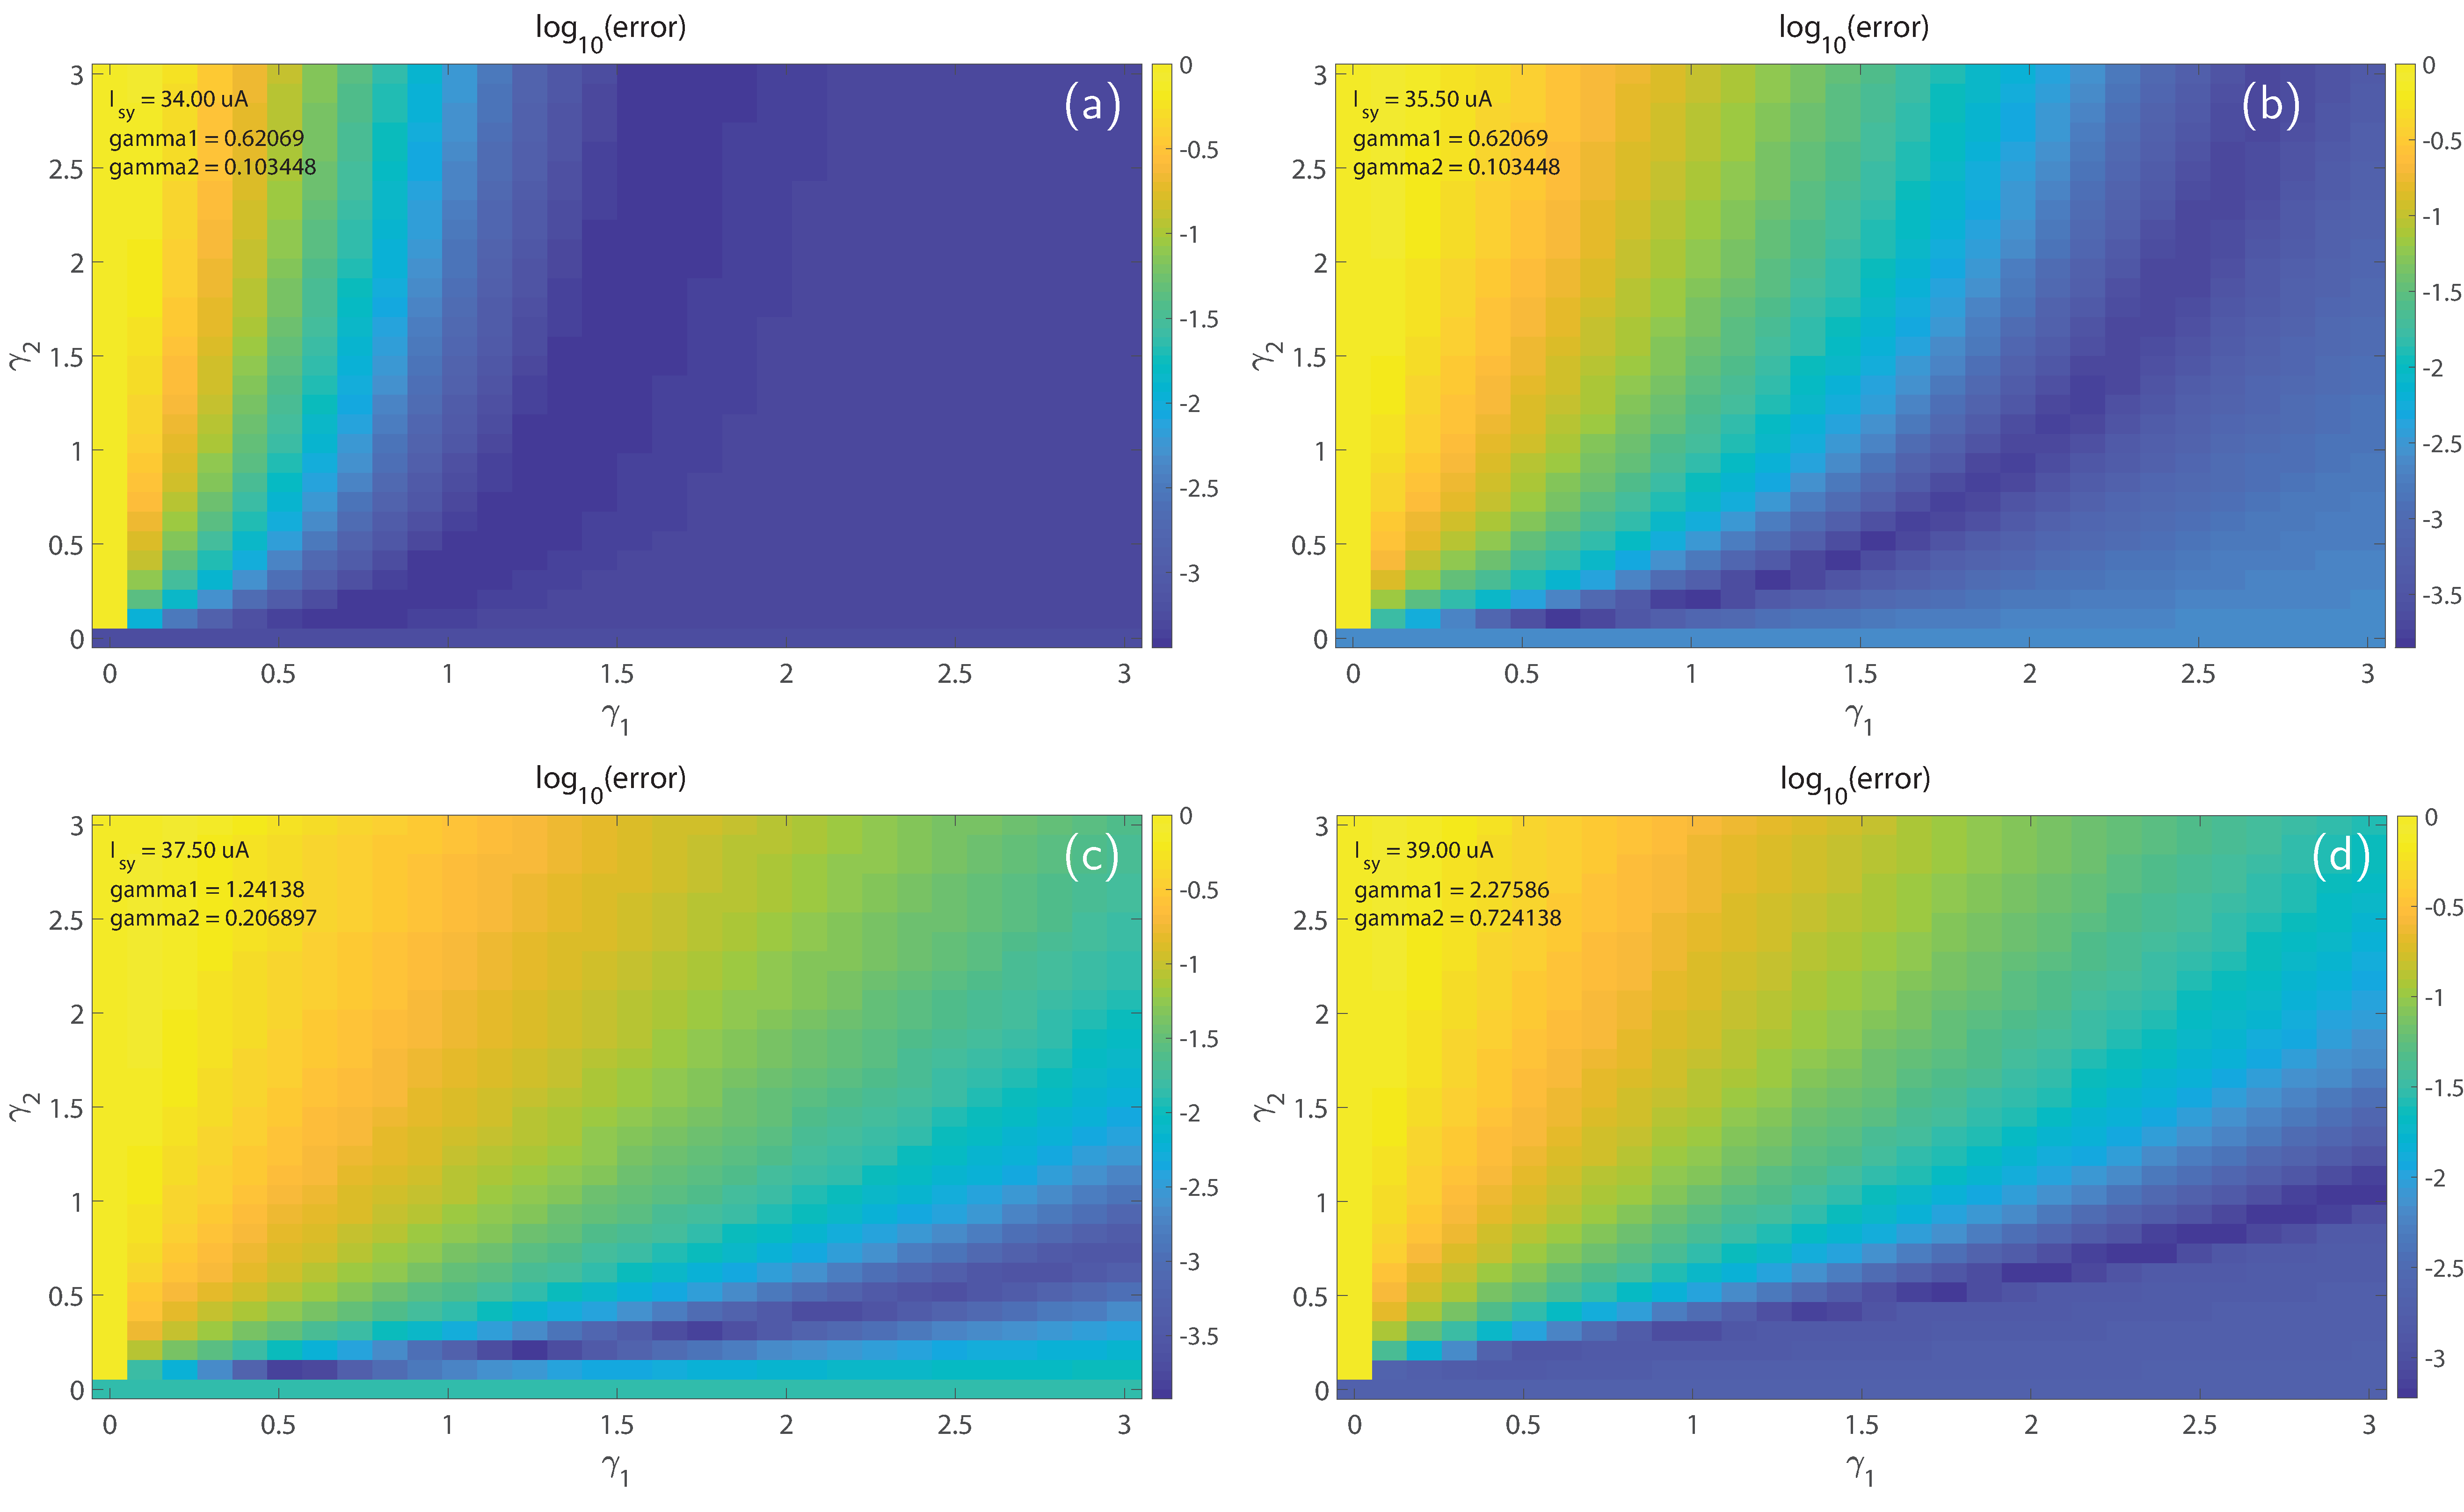
\includegraphics[width=17.2cm]{_finding_gammas.pdf}
%%\captionof{figure}{\label{fig:finding_gammas}Error as a function of $\gamma_1$ and $\gamma_2$. (a) $I_{sy} = 34$\,\textmu A. (b) $I_{sy} = 35.5$\,\textmu A. (c) $I_{sy} = 37.5$\,\textmu A. (d) $I_{sy} = 39$\,\textmu A. Note that we found $\gamma_1$ and $\gamma_2$ by finding decent fits for 11 values of $I_{sy}$ from 34\,\textmu A to 39\,\textmu A with $L_{si} = 50$\,nH and $r_{si} = 1\,\Omega$ and an input rate of synaptic firing events of 40\,MHz, but the values discovered provide good fits to behavior with all values of $I_{si}$, $L_{si}$, $r_{si}$, and input rate tested thus far. When determining $\gamma_1$ and $\gamma_2$, we used $\gamma_3 = 1$.}
%%\end{figure}
%To find $\gamma_1$, $\gamma_2$, and $\gamma_3$ I simulated the synaptic circuit across a range of operating conditions, calculated an error as a function of $\gamma_1$ and $\gamma_2$, and found values of these parameters that achieved low error for all operating conditions. The error is defined as
%\begin{equation}
%\label{eq:finding_gammas__error}
%E = \frac{\int_0^T\big|I_{si}^{\mathrm{circuit}}(t)-I_{si}^{\mathrm{model}}(t)\big|^2dt}{\int_0^T\big|I_{si}^{\mathrm{circuit}}(t)\big|^2dt},
%\end{equation}
%where $T$ is the duration of the time-domain circuit simulation attempting to be captured by the model. Example plots of error versus $\gamma_1$ and $\gamma_2$ are shown in Fig.\,\ref{fig:finding_gammas}.
%
%With $\gamma_1$ and $\gamma_2$ known, $\gamma_3$ was determined. $\gamma_3$ doesn't matter as much as the first two because the rise time of the post-synaptic response is much shorter than the fall time, so even an abrupt step provides a reasonable approximation to simulated circuit behavior. Nevertheless, using a fitting procedure similar to that used for $\gamma_1$ and $\gamma_2$, I find $\gamma_3 = 3/4$ does a good job in all cases considered here. The functional form of the rising term (Eq.\,\ref{eq:I_si__rising_term}) is not physically motivated or correct, but it is of little consequence for the intended purpose of the phenomenological model presented here.
%
%\section{\label{apx:dependence_of_I0_on_tau_si}Dependence of $I_0$ on $\tau_{si}$}
%%\begin{figure}[h!]
%%\centering
%%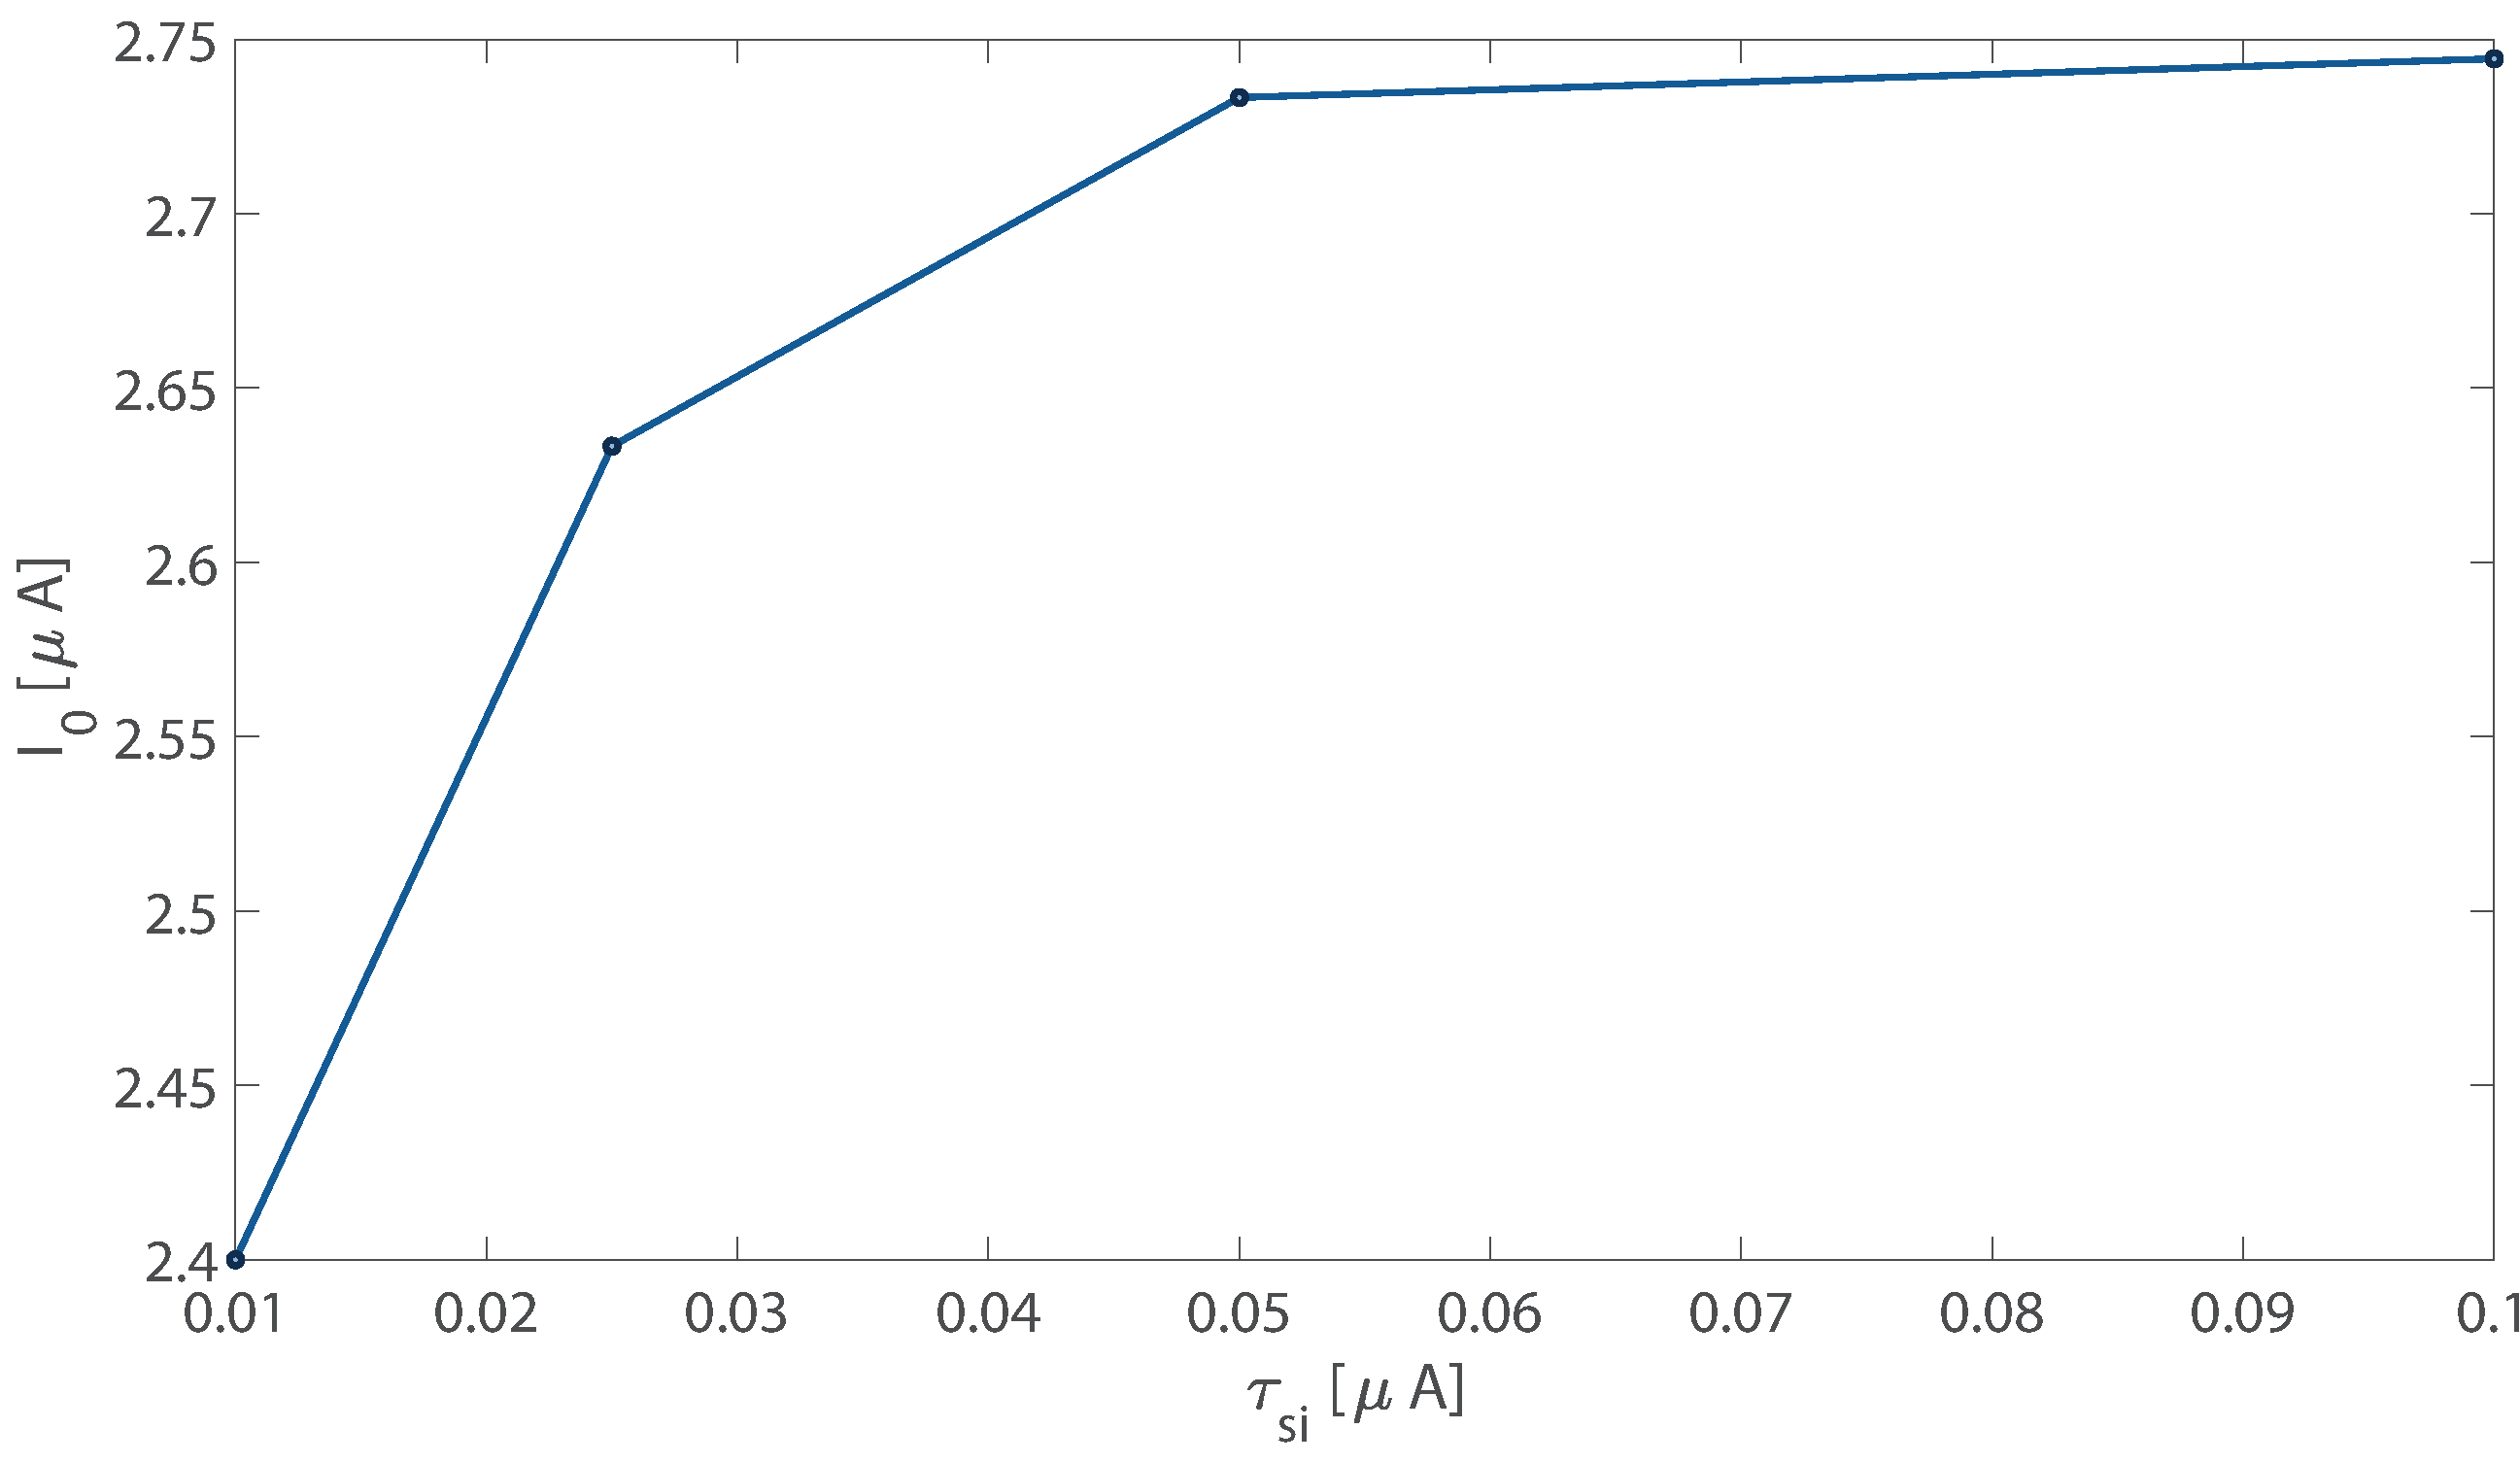
\includegraphics[width=17.2cm]{_I0_vs_tau_si.pdf}
%%\captionof{figure}{\label{fig:I0_vs_tau_si}Optimal $I_0$ as a function of $\tau_{si}$. For these simulations, $I_{sy} = 36.5$\,\textmu A and $L_{si} = 50$\,nH.}
%%\end{figure}
%The optimal value of $I_0$ is found to depend weakly on $\tau_{si}$ at very small $\tau_{si}$. Thus, the function given by Eq.\,\ref{eq:I0_vs_Isy} should also have a dependence on $\tau_{si}$. This is revealed in Fig.\,\ref{fig:I0_vs_tau_si}. However, this is a small effect that only matters for faster loops than I expect will be common. It can easily be handled if needed, but for now I neglect this dependency.

\bibliographystyle{unsrt}
\bibliography{phenomenological_modeling}

\end{document}